% Options for packages loaded elsewhere
\PassOptionsToPackage{unicode}{hyperref}
\PassOptionsToPackage{hyphens}{url}
\PassOptionsToPackage{dvipsnames,svgnames,x11names}{xcolor}
\documentclass[
]{article}
\usepackage{xcolor}
\usepackage[margin=25mm]{geometry}
\usepackage{amsmath,amssymb}
\setcounter{secnumdepth}{-\maxdimen} % remove section numbering
\usepackage{iftex}
\ifPDFTeX
  \usepackage[T1]{fontenc}
  \usepackage[utf8]{inputenc}
  \usepackage{textcomp} % provide euro and other symbols
\else % if luatex or xetex
  \usepackage{unicode-math} % this also loads fontspec
  \defaultfontfeatures{Scale=MatchLowercase}
  \defaultfontfeatures[\rmfamily]{Ligatures=TeX,Scale=1}
\fi
\usepackage{lmodern}
\ifPDFTeX\else
  % xetex/luatex font selection
\fi
% Use upquote if available, for straight quotes in verbatim environments
\IfFileExists{upquote.sty}{\usepackage{upquote}}{}
\IfFileExists{microtype.sty}{% use microtype if available
  \usepackage[]{microtype}
  \UseMicrotypeSet[protrusion]{basicmath} % disable protrusion for tt fonts
}{}
\makeatletter
\@ifundefined{KOMAClassName}{% if non-KOMA class
  \IfFileExists{parskip.sty}{%
    \usepackage{parskip}
  }{% else
    \setlength{\parindent}{0pt}
    \setlength{\parskip}{6pt plus 2pt minus 1pt}}
}{% if KOMA class
  \KOMAoptions{parskip=half}}
\makeatother
\usepackage{graphicx}
\makeatletter
\newsavebox\pandoc@box
\newcommand*\pandocbounded[1]{% scales image to fit in text height/width
  \sbox\pandoc@box{#1}%
  \Gscale@div\@tempa{\textheight}{\dimexpr\ht\pandoc@box+\dp\pandoc@box\relax}%
  \Gscale@div\@tempb{\linewidth}{\wd\pandoc@box}%
  \ifdim\@tempb\p@<\@tempa\p@\let\@tempa\@tempb\fi% select the smaller of both
  \ifdim\@tempa\p@<\p@\scalebox{\@tempa}{\usebox\pandoc@box}%
  \else\usebox{\pandoc@box}%
  \fi%
}
% Set default figure placement to htbp
\def\fps@figure{htbp}
\makeatother
\setlength{\emergencystretch}{3em} % prevent overfull lines
\providecommand{\tightlist}{%
  \setlength{\itemsep}{0pt}\setlength{\parskip}{0pt}}
\usepackage{bookmark}
\IfFileExists{xurl.sty}{\usepackage{xurl}}{} % add URL line breaks if available
\urlstyle{same}
\hypersetup{
  pdftitle={Ideal theory in rings},
  colorlinks=true,
  linkcolor={Maroon},
  filecolor={Maroon},
  citecolor={Blue},
  urlcolor={Blue},
  pdfcreator={LaTeX via pandoc}}

\title{Ideal theory in rings}
\author{}
\date{}

\begin{document}
\maketitle

{
\setcounter{tocdepth}{3}
\tableofcontents
}
\section{Chain conditions and irreducible
decompositions}\label{chain-conditions-and-irreducible-decompositions}

\emph{Written by GPT-6.1 Sol (OpenAI) in Codex at Ultra reasoning
effort, October 2026. Self-checked by the writing AI, GPT-6.1 Sol, at
Ultra. No independent review is claimed. Public domain (CC0).}

Factoring an integer produces canonical prime powers. Intersecting
ideals produces a different kind of arithmetic: components can move
while their number remains fixed. We will discover the invariant first
through the lattice of submodules and then through vector spaces called
socles. This also explains why embedded components contribute to the
count.

We assume rings are commutative with identity. A proper ideal is
\textbf{irreducible} if it cannot be written as the intersection of two
strictly larger ideals. This is irreducibility for intersection, rather
than for multiplication. The earlier lesson
\href{../prerequisites/AG-CA/AG-CA-03.html}{Noetherian and Artinian
rings} proves the chain-condition equivalences in Theorem 1.1, the
finite-module consequences in Proposition 1.2, and the Hilbert basis
theorem in Theorem 2.1.
\href{../prerequisites/AG-CA/AG-CA-02.html}{Localization, local
properties and support}, Theorems 2.1 and 3.1, proves exactness,
preservation of finite intersections and the prime correspondence. For
Section 4 we use the actual proofs in
\href{../prerequisites/AG-CA/AG-CA-04.html}{Associated primes and
primary decomposition}: Theorem 1.2 for existence and zero divisors,
Proposition 2.1 for submodules and direct sums, Theorem 2.2 for
finiteness, Theorems 3.1--3.2 for localization and support, and
Proposition 4.1 for primary finite modules. The decomposition and
counting arguments below are proved here. Freely accessible references
are Noether's English working edition and the Stacks project.

\subsection{1. The example that asks the
question}\label{the-example-that-asks-the-question}

In \(k[x,y]\), for every \(a\in k\),

\[
(x^2,xy)=(x)\cap(x^2,y+ax).
\]

Indeed, substitute \(y=-ax\) modulo the second ideal. If \(xf\) lies in
that ideal, its image in \(k[x]/(x^2)\) vanishes, so the constant term
of \(f(x,-ax)\) is zero. Hence \(f\in(x,y)\) and \(xf\in(x^2,xy)\). The
converse inclusion follows from the generators. The ideal \((x)\) is
prime. The other quotient is \(k[x]/(x^2)\), whose nonzero ideals all
contain the class of \(x\). Its zero ideal is therefore irreducible.
Neither component contains the other: \(x\) is missing from the second
and \(y+ax\) from the first. The decomposition is irredundant.

The embedded component varies with \(a\). Over an infinite field there
are infinitely many choices. Nevertheless each decomposition has two
components. The count will turn out to measure an intrinsic property of
the quotient.

\subsection{2. Induction without a numerical
size}\label{induction-without-a-numerical-size}

\textbf{Theorem 2.1 (Noetherian induction).} Suppose ideals of \(R\)
satisfy the ascending chain condition. If a property holds for \(I\)
whenever it holds for all ideals strictly containing \(I\), it holds for
every ideal.

\textbf{Proof.} If failures existed, the maximal condition would give a
maximal failing ideal \(I\). All larger ideals would satisfy the
property, forcing it for \(I\) too. This is a contradiction. \(\square\)

\textbf{Theorem 2.2 (finite irreducible decomposition).} Every proper
submodule \(N\) of a Noetherian module \(M\) is a finite intersection of
irreducible proper submodules. In particular this holds for ideals of a
Noetherian ring.

\textbf{Proof.} Apply the same maximal-counterexample argument in the
submodule lattice. A maximal failure \(N\) cannot be irreducible,
because a one-component decomposition would suffice. Write \(N=A\cap B\)
with \(A,B\supsetneq N\). Maximality gives finite decompositions of
\(A\) and \(B\), and combining them gives one of \(N\). Remove redundant
factors. \(\square\)

The largest submodule is the empty intersection; it has zero components.
We reserve the word irreducible for proper submodules.

These arguments need the chain condition, not a polynomial presentation.
Here are four ways that condition can fail.

\begin{itemize}
\tightlist
\item
  In \(k[x_1,x_2,\ldots]\), the ideals \((x_1,\ldots,x_n)\) strictly
  increase.
\item
  In \(k[x,xy,xy^2,\ldots]\), the ideals generated by
  \(x,xy,\ldots,xy^n\) strictly increase: their terms of \(x\)-degree
  one have \(y\)-degree at most \(n\), while products with nonconstant
  ring elements increase the \(x\)-degree.
\item
  In the ring of all algebraic integers,
  \((2)\subsetneq(2^{1/2})\subsetneq(2^{1/4})\subsetneq\cdots\). The
  reverse quotient \(2^{-1/2^n}\) is not an algebraic integer: a
  positive power is \(1/2\), which is not an integer although a rational
  algebraic integer must be one.
\item
  In \(C([0,1],\mathbb R)\), put \(f_n(t)=t^{1/2^n}\). Then
  \((f_n)\subsetneq(f_{n+1})\); expressing \(f_{n+1}\) as a continuous
  multiple of \(f_n\) would require a function unbounded at zero.
\end{itemize}

The integrality fact in the third example has a short direct proof. If
\(\alpha\) satisfies a monic integer polynomial of degree \(d\), then
\(\mathbb Z[\alpha]\) is generated over \(\mathbb Z\) by
\(1,\alpha,\ldots,\alpha^{d-1}\). Multiplication by any
\(\beta\in\mathbb Z[\alpha]\) is represented on these generators by an
integer matrix \(B\). The adjugate identity for \(XI-B\), evaluated at
\(\beta\), shows that its monic determinant annihilates all generators,
including \(1\). Thus every power of an algebraic integer is integral.
If a reduced rational \(a/b\), with \(b>0\), satisfies a monic equation
of degree \(d\), clearing denominators gives \(b\mid a^d\), hence
\(b=1\). This excludes \(1/2\) and therefore every \(2^{-1/2^n}\).

\subsection{3. The lattice mechanism}\label{the-lattice-mechanism}

A lattice has a meet \(u\wedge v\) and a join \(u\vee v\). It is
\textbf{modular} if

\[
u\vee(v\wedge w)=(u\vee v)\wedge w\qquad(u\leq w).
\]

\textbf{Proposition 3.1.} Submodules form a modular lattice, with meet
intersection and join sum.

\textbf{Proof.} Assume \(A\subset C\). The inclusion
\(A+(B\cap C)\subset(A+B)\cap C\) is immediate. For the reverse, if
\(z=a+b\in C\), then \(b=z-a\in C\), so \(b\in B\cap C\). \(\square\)

\textbf{Lemma 3.2 (transposition).} In a modular lattice, put
\(a=b\wedge c\). The maps

\[
[a,b]\longrightarrow[c,b\vee c],\quad x\longmapsto x\vee c,
\qquad z\longmapsto z\wedge b
\]

are mutually inverse order isomorphisms.

\textbf{Proof.} For \(a\le x\le b\), modularity gives
\((x\vee c)\wedge b=x\vee(c\wedge b)=x\). For \(c\le z\le b\vee c\), it
gives \(c\vee(z\wedge b)=z\wedge(c\vee b)=z\). Both maps preserve order.
An order isomorphism preserves meets and joins taken within these
intervals. \(\square\)

Call an interval \([a,b]\) \textbf{uniform above \(a\)} when two
elements in it strictly above \(a\) have meet strictly above \(a\). If
\(c\) is meet-irreducible, the interval \([c,b\vee c]\) is uniform above
\(c\). Lemma 3.2 transports this to \([a,b]\). Thus

\[
b\wedge c=a,\ c\text{ meet-irreducible}
\quad\Longrightarrow\quad
\bigwedge_{j=1}^s x_j=a,\ x_j\in[a,b]
\ \Longrightarrow\ x_j=a\text{ for some }j.
\]

The implication also holds if \(b=a\). For a nonsingleton interval,
induction on \(s\) proves it from the binary condition.

\textbf{Theorem 3.3 (exchange and the Kurosh--Ore count).} Suppose a
modular lattice has finite decompositions

\[
a=\bigwedge_{i=1}^m b_i=\bigwedge_{j=1}^n c_j.
\]

If every \(b_i\) is meet-irreducible, then each \(b_i\) can be exchanged
for some \(c_j\): with \(B_i=\bigwedge_{k\ne i}b_k\), one has
\(a=B_i\wedge c_j\). If both decompositions are irredundant and all
their components are meet-irreducible, then \(m=n\).

\textbf{Proof.} All the elements \(B_i\wedge c_j\) lie in \([a,B_i]\),
and their meet is \(a\). This interval is uniform by the preceding
consequence of transposition, since \(B_i\wedge b_i=a\). Therefore one
of them equals \(a\), proving exchange.

Replace \(b_1\), then \(b_2\), and so forth using this argument. At each
stage the component about to be replaced is still one of the original
meet-irreducible \(b_i\), and the meet of all current components is
\(a\). The intermediate list need not initially be assumed irredundant.
After \(m\) replacements, a sublist of at most \(m\) of the \(c_j\) has
meet \(a\). Irredundancy of their original list forces all \(n\)
distinct components to occur, so \(n\le m\). Reverse the roles to get
\(m\le n\).

In fact every intermediate list is irredundant. If one had fewer than
\(m=n\) necessary components, delete the others and apply the same
replacement argument to that list and the original \(c_j\). It would
imply \(n<m\), a contradiction. \(\square\)

The ascending chain condition guarantees existence of finite
decompositions by Theorem 2.2's lattice argument. Once finite
decompositions exist, their count needs only modularity. Noether proved
the ideal version in 1921; the modular-lattice theorem bears the names
of Kurosh and Ore.

\textbf{Lemma 3.4 (primary quotients).} An irreducible submodule of a
Noetherian module over a commutative ring is primary: multiplication by
each scalar on its quotient is injective or nilpotent.

\textbf{Proof.} Its nonzero quotient \(U\) is uniform. If multiplication
by \(a\) has nonzero kernel, the ascending chain \(0:_U a^j\) stabilizes
at some \(h\ge1\). Then \(a^hU\cap(0:_U a^h)=0\): if \(a^{2h}u=0\),
stabilization gives \(a^hu=0\). Since the second submodule is nonzero,
uniformity forces \(a^hU=0\). This proves the assertion. \(\square\)

\subsection{4. Local vector spaces that count the
components}\label{local-vector-spaces-that-count-the-components}

Lemma 3.4 makes the irreducible quotients primary. Here is how its
scalar condition identifies the prime. For a nonzero finite quotient
\(U\) satisfying that condition, let \(J=\sqrt{\operatorname{Ann}(U)}\).
A scalar is noninjective precisely when it belongs to \(J\): Lemma 3.4
proves one implication, and an injective nilpotent endomorphism of a
nonzero module is impossible. By the earlier existence theorem choose
\(\mathfrak p=\operatorname{Ann}(u)\) with \(u\ne0\). Every element of
\(\mathfrak p\) is noninjective, so \(\mathfrak p\subset J\); conversely
\(\operatorname{Ann}(U)\subset\mathfrak p\) gives
\(J\subset\mathfrak p\). Thus \(J=\mathfrak p\) is prime and is the only
associated prime. Elements outside it act injectively. A power of this
ideal kills \(U\): choose generators \(a_i\) and powers
\(a_i^{e_i}U=0\); every product of \(1+\sum_i(e_i-1)\) generators
contains a vanishing power. For the zero ideal its first power suffices.
The earlier associated-prime localization theorem is used below.

The \textbf{socle} of a module over a local ring \((A,\mathfrak m)\) is

\[
\operatorname{Soc}(U)=0:_U\mathfrak m
\cong\operatorname{Hom}_A(A/\mathfrak m,U).
\]

It is a vector space over the residue field. A submodule \(E\subset U\)
is \textbf{essential} if it meets every nonzero submodule nontrivially.
A module is \textbf{uniform} if any two nonzero submodules meet
nontrivially. The zero submodule is irreducible exactly when its
quotient is uniform.

\textbf{Lemma 4.1.} A nonzero finite-length module over a local ring has
essential socle. It is uniform exactly when its socle has dimension one.

\textbf{Proof.} Every nonzero submodule has a simple submodule, by
choosing one of minimal positive length. A simple module over a local
ring \((A,\mathfrak m)\) is generated by any nonzero element \(v\); it
is \(A/\operatorname{Ann}(v)\), and simplicity makes that annihilator
maximal. Thus it is the residue field and lies in the socle. If the
socle has dimension one, all nonzero submodules contain it and
intersect. If the dimension is at least two, distinct one-dimensional
subspaces are submodules with zero intersection. \(\square\)

\textbf{Lemma 4.2.} If \(U\) is a finite primary quotient with
associated prime \(\mathfrak p\), then \(U\to U_{\mathfrak p}\) is
injective. Moreover \(U\) is uniform if and only if \(U_{\mathfrak p}\)
is uniform.

\textbf{Proof.} Every denominator outside \(\mathfrak p\) acts
injectively, so \(U\to U_{\mathfrak p}\) is injective and nonzero
submodules stay nonzero. If \(U_{\mathfrak p}\) is uniform, the
localizations of two nonzero submodules of \(U\) intersect nontrivially.
Exactness identifies this intersection with the localization of their
intersection, so that original intersection is nonzero. Conversely, let
\(U\) be uniform and let \(H,K\subset U_{\mathfrak p}\) be nonzero.
Multiplying a nonzero fraction in each by its denominator gives nonzero
elements in their contractions to \(U\). These contractions have nonzero
intersection by uniformity; injectivity keeps a nonzero element of that
intersection nonzero after localization. It belongs to \(H\cap K\).
\(\square\)

Since a power of \(\mathfrak p\) kills \(U\), its localization has
finite length: the finite filtration by powers of the local maximal
ideal has finite-dimensional residue-field vector spaces as its
successive quotients. Lemmas 4.1--4.2 therefore show that a
\(\mathfrak p\)-primary submodule is irreducible exactly when its
localized quotient has one-dimensional socle.

\textbf{Theorem 4.3 (socle count).} Let \(M\) be a finite module over a
Noetherian ring, and let \(N=\bigcap_{i=1}^r Q_i\) be an irredundant
irreducible decomposition. For every prime \(\mathfrak p\),

\[
\#\{i:\operatorname{Ass}(M/Q_i)=\{\mathfrak p\}\}
=\dim_{\kappa(\mathfrak p)}
\operatorname{Soc}((M/N)_{\mathfrak p}).
\]

\textbf{Proof.} The diagonal injection

\[
D=M/N\hookrightarrow E=\bigoplus_i M/Q_i
\]

has essential image. To see this, for each \(i\) the complement
intersection \(\bigcap_{j\ne i}Q_j\) maps to a nonzero submodule \(K_i\)
of the \(i\)-th summand, and to zero in the other summands. Irredundancy
gives nonzeroness. Each summand is uniform, so \(K_i\) is essential in
it. The direct sum \(\bigoplus K_i\subset D\) is essential in \(E\).
Indeed, start with a nonzero submodule \(H\subset E\) and impose
membership in \(K_1,K_2,\ldots\), one coordinate at a time. If the next
projection of the current nonzero submodule is zero, it already meets
that condition. Otherwise essentiality supplies a scalar multiple of
some projected element that is nonzero in \(K_i\); the same scalar
multiple of its lift is nonzero and satisfies the new condition. Earlier
conditions are preserved because the \(K_j\) are submodules. After
finitely many steps \(H\) meets \(\bigoplus K_i\) nontrivially.

Essentiality survives localization here. Indeed, if a nonzero submodule
\(H\subset E_{\mathfrak p}\) had zero intersection with
\(D_{\mathfrak p}\), contract it to \(L\subset E\). Every element of
\(L\cap D\) is killed by some denominator outside \(\mathfrak p\). This
intersection is finitely generated, so one common denominator
\(s\notin\mathfrak p\) kills it. The ascending sequence \(0:_L s^t\)
stabilizes, say at \(t=h\). The nonzero submodule \(s^hL\) would have
zero intersection with \(D\): an element in that intersection is killed
by \(s\), so stabilization makes it zero. It is nonzero since its
localization is \(H\). This contradicts essentiality.

Every simple submodule of \(E_{\mathfrak p}\) must then lie in
\(D_{\mathfrak p}\), so their socles coincide. A summand with associated
prime \(\mathfrak q\) vanishes if \(\mathfrak q\not\subset\mathfrak p\).
If \(\mathfrak q\subsetneq\mathfrak p\), choose
\(a\in\mathfrak p\setminus\mathfrak q\); it acts injectively, so that
summand has zero \(\mathfrak p\)-socle. If \(\mathfrak q=\mathfrak p\),
Lemmas 4.1--4.2 give a socle of dimension one. Adding these dimensions
proves the formula. \(\square\)

For ideals take \(M=R\). The socle count is also called the zeroth Bass
number. It vanishes for primes not associated to \(M/N\), by the
localization rule for associated primes.

\subsection{5. Computations and a failure without
finiteness}\label{computations-and-a-failure-without-finiteness}

For \(I=(x^2,xy)\), localization at \((x)\) makes \(y\) invertible and
yields the residue field of \(R_{(x)}\), so its socle has dimension one.
At \((x,y)\), the socle is spanned by \(x\). Indeed every localized
class has the form \(f(y)+cx\), with \(f\in k[y]_{(y)}\) and \(c\in k\);
multiplication by \(y\) forces \(f=0\). Thus there is one component at
each of these two associated primes.

For \(I=(x,y)^2\), the quotient has basis \(1,x,y\) and socle
\(kx\oplus ky\). Direct monomial membership gives

\[
(x,y)^2=(x^2,y)\cap(x,y^2).
\]

Each quotient has one-dimensional socle. For \(J=(x^2,xy^3,y^4)\), the
standard monomials are \(1,y,y^2,y^3,x,xy,xy^2\). Its socle has basis
\(y^3,xy^2\), and

\[
J=(x^2,y^3)\cap(x,y^4).
\]

The rule behind this staircase calculation is proved in
\href{../NOE-IDL-03.html}{Modules, staircases and elementary divisors},
Section 2.

Finally let \(R=\prod_{n\ge1}k\). Its zero ideal has no finite
irreducible decomposition. Otherwise \(R\) would embed in a sum of
finitely many uniform quotients. To justify the obstruction, note that
every quotient is again a commutative von Neumann regular ring: the
coordinatewise inverse on nonzero coordinates gives \(a=a^2b\), and this
identity descends. In a uniform such ring each principal ideal is
generated by an idempotent \(e=ab\); the ideals \((e)\) and \((1-e)\)
have zero intersection, so every nonzero idempotent is \(1\). Hence a
nonzero element is a unit and the quotient is a field. Each map from
\(R\) to a field sends at most one of the mutually orthogonal coordinate
idempotents to a nonzero element. Finitely many maps therefore kill some
nonzero coordinate idempotent, contradicting injectivity.

\subsection{6. Exercises}\label{exercises}

\begin{enumerate}
\def\labelenumi{\arabic{enumi}.}
\tightlist
\item
  \textbf{Basic.} Prove that prime ideals are irreducible. Give an
  irreducible ideal which is not prime.
\item
  \textbf{Intermediate.} Compute an irredundant decomposition of
  \((x^2,xy^3,y^4)\) into ideals generated by powers of variables, and
  justify irreducibility of the factors.
\item
  \textbf{Intermediate.} Prove the modular law for submodules and give a
  nonmodular lattice.
\item
  \textbf{Intermediate.} Compute the socle of \(k[x,y]/(x^3,x^2y,y^2)\),
  and an irreducible decomposition of its defining ideal.
\item
  \textbf{Advanced.} Explain why exchange in Theorem 3.3 still works if
  the second decomposition has arbitrary components; then prove the
  count without assuming that intermediate replacement lists are
  irredundant.
\end{enumerate}

\subsection{7. Solutions}\label{solutions}

\textbf{1.} If \(\mathfrak p=A\cap B\) and both ideals are larger,
choose \(a\in A\setminus\mathfrak p\) and
\(b\in B\setminus\mathfrak p\). Then \(ab\in A\cap B=\mathfrak p\),
contrary to primality. The ideal \((t^2)\subset k[t]\) is irreducible
since every nonzero ideal of its quotient contains \(\bar t\); it is not
prime since \(t^2\in(t^2)\) but \(t\notin(t^2)\).

\textbf{2.} The answer is \((x^2,y^3)\cap(x,y^4)\). Membership in the
intersection means either an \(x\)-exponent at least two, or positive
\(x\)-exponent and \(y\)-exponent at least three, or \(y\)-exponent at
least four. These are exactly the three generating alternatives. Both
quotients are local Artinian with one-dimensional socle, respectively
spanned by \(xy^2\) and \(y^3\), so Lemma 4.1 gives irreducibility. The
monomials \(x\) and \(y^3\) show neither factor can be omitted.

\textbf{3.} For \(A\subset C\), an element \(a+b\in(A+B)\cap C\) has
\(b\in B\cap C\), proving the law. In the pentagon lattice \(0<a<c<1\),
\(0<b<1\), with \(a,b\) and \(c,b\) incomparable, take \(u=a,v=b,w=c\).
Then \(u\vee(v\wedge w)=a\) while \((u\vee v)\wedge w=c\).

\textbf{4.} The standard basis is \(1,x,x^2,y,xy\). The elements killed
by both \(x\) and \(y\) are precisely \(kx^2\oplus kxy\). Thus there are
two components, and termwise membership verifies

\[
(x^3,x^2y,y^2)=(x^3,y)\cap(x^2,y^2).
\]

Their socles are spanned by \(x^2\) and \(xy\). The witnesses \(y\) and
\(x^2\) establish irredundancy.

\textbf{5.} In \([a,B_i]\) the finitely many elements \(B_i\wedge c_j\)
meet to \(a\). Uniformity depends only on the irreducibility of \(b_i\),
so some intersection equals \(a\), without a condition on \(c_j\).
Replacing all \(m\) of the original components produces a sublist of at
most \(m\) of the second list. If the second list is irredundant it must
be exhausted, giving \(n\le m\). Reverse the process for the reverse
inequality. The argument never used irredundancy of an intermediate
list.

\subsection{In Noether's words}\label{in-noethers-words}

Noether's 1921 paper treats intersections as least common multiples and
sums as greatest common divisors. Her divisibility convention reverses
containment. Sections 2--3 establish finite irreducible decompositions
and equality of their counts. Her rings may have no identity; our unital
convention becomes important for the residue-field and socle language.
The entire work can be read in the
\href{https://github.com/KokunoYumeto/emmy-noether-en/blob/main/source/Noether_English_ED0014.tex}{linked
English edition, work 19} alongside the
\href{https://doi.org/10.5281/zenodo.21908301}{German authority
edition}. Those linked editions retain their own rights and provenance.

\subsection{References}\label{references}

\begin{itemize}
\tightlist
\item
  Emmy Noether, \emph{Idealtheorie in Ringbereichen}, 1921, introduction
  and Sections 1--4, 9.
  \href{https://github.com/KokunoYumeto/emmy-noether-en/blob/main/source/Noether_English_ED0014.tex}{Free
  English working edition, work 19}, with the original bibliographic
  information and machine-assisted translation provenance.
\item
  The Stacks project authors, Noetherian rings and associated primes:
  \href{https://kokunoyumeto.github.io/stacks-zh-hans-cn/en/algebra.html\#section-Noetherian}{Tag
  00FM},
  \href{https://kokunoyumeto.github.io/stacks-zh-hans-cn/en/algebra.html\#lemma-Noetherian-permanence}{Tag
  00FN},
  \href{https://kokunoyumeto.github.io/stacks-zh-hans-cn/en/algebra.html\#section-ass}{Tag
  00L9}. The \href{https://stacks.math.columbia.edu/}{official Stacks
  project} is the original work. These tag links use AI Integrated
  Stacks Project, an edition with AI-proposed corrections and AI-written
  additions, not reviewed by the Stacks project's maintainers. The
  source text is GFDL; this lesson independently states its mathematics.
\end{itemize}

\subsection{Editable sources}\label{editable-sources}

\href{ideal-theory-in-rings-source.zip}{Complete source archive} ·
\href{ideal-theory-in-rings.tex}{Complete course in LaTeX} ·
\href{NOE-IDL-01.tex}{This lesson in LaTeX}. The archive includes all
five lesson texts, the figures and their reproducible source.

\section{Primary ideals and isolated
components}\label{primary-ideals-and-isolated-components}

\emph{Written by GPT-6.1 Sol (OpenAI) in Codex at Ultra reasoning
effort, October 2026. Self-checked by the writing AI, GPT-6.1 Sol, at
Ultra. No independent review is claimed. Public domain (CC0).}

An irreducible intersection decomposition need not be unique. We now ask
what can still be recovered without choosing a decomposition.
Localization singles out groups of primary components. A second
construction groups associated primes by containment; a third groups the
actual connected pieces of the spectrum. These are different kinds of
separation.

We assume a Noetherian commutative ring \(R\) with identity. We use the
finite irreducible decompositions proved in
\href{../NOE-IDL-01.html}{Chain conditions and irreducible
decompositions}. The earlier lesson
\href{../prerequisites/AG-CA/AG-CA-04.html}{Associated primes and
primary decomposition} contains actual proofs of associated-prime
existence and zero divisors (Theorem 1.2), submodule and direct-sum
inclusions (Proposition 2.1), finiteness (Theorem 2.2), localization and
minimal support (Theorems 3.1--3.2), primary modules and ideals
(Proposition 4.1 and Theorem 4.2), primary-decomposition existence
(Theorem 5.3), and uniqueness (Theorems 6.1--6.2). We use those results
with their Noetherian and finite-module hypotheses. Finite prime
avoidance and the Chinese remainder construction are proved below.
\href{../prerequisites/AG-CA/AG-CA-01.html}{Spectra of rings}, Theorem
1.2, Proposition 2.1 and Theorems 4.1 and 4.3, proves the radical
correspondence, closed-set operations and finite irreducible components;
\href{../prerequisites/AG-CA/AG-CA-03.html}{Noetherian and Artinian
rings}, Proposition 2.2, proves nilradical nilpotence. Freely accessible
references are Noether's English working edition and the Stacks project.

\subsection{1. The chain argument that makes a component
primary}\label{the-chain-argument-that-makes-a-component-primary}

An ideal \(Q\ne R\) is \textbf{primary} if \(ab\in Q\) and \(b\notin Q\)
imply \(a^n\in Q\) for some \(n\ge1\). Its radical is a prime. For a
submodule \(N\ne M\), the corresponding condition is that \(av\in N\),
\(v\notin N\) imply \(a^nM\subset N\). Equivalently, multiplication by
each scalar on \(M/N\) is either injective or nilpotent. These
conditions agree for ideals, using finite generation to pass from
individual powers to a common power.

\textbf{Theorem 1.1 (Noether's primary lemma).} An irreducible submodule
of a Noetherian module over a commutative ring is primary.

\textbf{Proof.} Pass to \(U=M/N\), so zero is irreducible and \(U\) is
uniform. Fix \(a\in R\) whose multiplication map has a nonzero kernel.
The ascending chain \(0:_U a^j\) stabilizes, say at \(j=h\ge1\). The
submodules \(a^hU\) and \(0:_U a^h\) intersect trivially: if \(a^hu\)
lies in the latter, then \(a^{2h}u=0\), so stabilization implies
\(a^hu=0\). The kernel submodule is nonzero. Uniformity therefore forces
\(a^hU=0\). Thus every noninjective scalar is nilpotent on \(U\), as
required. \(\square\)

In the ideal version, if \(ab\in Q\) with \(b\notin Q\), choose \(h\)
with \((Q:a^h)=(Q:a^{2h})\). Then

\[
Q=(Q+a^hR)\cap(Q+bR).
\]

For if \(z=q+a^hr=q'+bs\), multiplication by \(a\) gives
\(a^{h+1}r\in Q\), since \(ab\in Q\). Stabilization gives \(a^hr\in Q\),
so \(z\in Q\). Irreducibility and \(b\notin Q\) force \(a^h\in Q\). This
is the scalar form of the same proof.

Together with finite irreducible decompositions this gives Noether's
existence route to primary decomposition. The associated-prime route and
the classical uniqueness statements are the cited prerequisite theorems.
We now prove the further uniqueness statements specific to this lesson.

\subsection{2. Selecting an entire isolated
set}\label{selecting-an-entire-isolated-set}

\textbf{Lemma 2.0 (finite prime avoidance).} Let \(J,I_1,\ldots,I_r\) be
ideals of a commutative ring, with all but at most two of the \(I_i\)
prime. If \(J\not\subset I_i\) for every \(i\), there is
\(a\in J\setminus\bigcup_i I_i\). In particular, if an ideal is
contained in a finite union of prime ideals, it is contained in one of
them.

\textbf{Proof.} For \(r=0\), choose \(a=0\); for \(r=1\), the assertion
is the hypothesis. For \(r=2\), choose \(x\in J\setminus I_1\) and
\(y\in J\setminus I_2\). If neither already avoids both, then
\(x\in I_2\) and \(y\in I_1\), and \(x+y\) avoids both by subtraction.

Induct on \(r\). Delete an ideal contained in another: this changes
neither the union nor the desired conclusion. If deletion reduces the
list, use induction. Otherwise there are no inclusions, and for
\(r\ge3\) we may put a prime ideal last. Induction gives \(x\in J\)
outside \(I_1,\ldots,I_{r-1}\). If \(x\notin I_r\), it works. Otherwise
choose \(b\in J\setminus I_r\) and, for each \(i<r\), choose
\(b_i\in I_i\setminus I_r\), using noncontainment. Set
\(y=b\prod_{i<r}b_i\). Then \(y\in J\cap\bigcap_{i<r}I_i\), while
primality gives \(y\notin I_r\). For \(i<r\), membership of \(x+y\) in
\(I_i\) would force \(x\in I_i\); membership in \(I_r\) would force
\(y\in I_r\). Thus \(x+y\) avoids the entire list. The last assertion is
the contrapositive for a list of prime ideals. \(\square\)

Fix a primary decomposition

\[
I=\bigcap_{\mathfrak p\in P}Q_{\mathfrak p},
\qquad P=\operatorname{Ass}(R/I),
\]

with distinct radicals and no redundant component. A subset
\(S\subset P\) is \textbf{isolated} if
\(\mathfrak q\subset\mathfrak p\), \(\mathfrak q\in P\),
\(\mathfrak p\in S\) imply \(\mathfrak q\in S\). This is downward
closure within the finite associated set; it does not ask that every
prime of \(R\) below \(\mathfrak p\) belong to \(P\).

\textbf{Theorem 2.1.} Put
\(T=R\setminus\bigcup_{\mathfrak p\in S}\mathfrak p\). Then

\[
I_S:=\bigcap_{\mathfrak p\in S}Q_{\mathfrak p}
=\{r\in R:r/1\in I R_T\}.
\]

In particular \(I_S\) is independent of the chosen primary
decomposition.

\textbf{Proof.} The set \(T\) is multiplicatively closed. For a
\(\mathfrak q\)-primary ideal \(Q\), if
\(T\cap\mathfrak q\ne\varnothing\), a power of an element of this
intersection lies in \(Q\), so \(QR_T=R_T\). If
\(T\cap\mathfrak q=\varnothing\), the contraction of \(QR_T\) is exactly
\(Q\): from \(tr\in Q\) and \(t\notin\mathfrak q\), primaryness gives
\(r\in Q\).

The primes of \(P\) disjoint from \(T\) are exactly those in \(S\). One
inclusion is immediate. For the other, disjointness says
\(\mathfrak q\subset\bigcup_{\mathfrak p\in S}\mathfrak p\). Lemma 2.0
puts \(\mathfrak q\) inside one of those primes, and isolation puts it
in \(S\). Localization preserves finite intersections, so only the
selected components survive, with their contractions unchanged. This
proves the formula. If \(S=\varnothing\), take \(T=R\), which contains
zero; the localization is zero and the contraction is \(R\), agreeing
with the empty intersection. \(\square\)

For \((x^2,xy)\), the associated primes are \((x)\subset(x,y)\). The set
consisting of \((x)\) is isolated, and localization gives
\(I_{\{(x)\}}=(x)\). The singleton consisting of \((x,y)\) is not
isolated; the component \((x^2,y+ax)\) can vary.

\subsection{3. Relative primality is
directional}\label{relative-primality-is-directional}

Define the ideal quotient \((B:A)=\{r:rA\subset B\}\). Say that \(A\) is
\textbf{relatively prime to \(B\)} if \((B:A)=B\). This means that the
entire ideal \(A\) kills no nonzero element of \(R/B\). Say
\textbf{mutually relatively prime} when both directions hold. These
words do not mean comaximal.

\textbf{Theorem 3.1.} For \(B\ne R\), the following are equivalent:

\begin{enumerate}
\def\labelenumi{\arabic{enumi}.}
\tightlist
\item
  \((B:A)=B\).
\item
  \(A\) is contained in no prime of \(\operatorname{Ass}(R/B)\).
\item
  No prime of \(\operatorname{Ass}(R/A)\) is contained in a prime of
  \(\operatorname{Ass}(R/B)\).
\end{enumerate}

\textbf{Proof.} If \(A\subset\mathfrak p=\operatorname{Ann}(v)\) for a
nonzero \(v\in R/B\), then \(Av=0\), so the ideal quotient is larger
than \(B\). Conversely, if \(K=0:_{R/B}A\ne0\), it has an associated
prime \(\mathfrak p\), and an element of \(K\) with that annihilator is
also in \(R/B\). Necessarily \(A\subset\mathfrak p\). This proves
equivalence of the first two conditions. For any prime \(\mathfrak p\)
containing \(A\), there is a minimal prime \(\mathfrak q\) over \(A\)
contained in \(\mathfrak p\) (Spectra of rings, Lemma 4.2), and this
\(\mathfrak q\) is associated to \(R/A\) (Associated primes and primary
decomposition, Theorem 3.2). Conversely every associated prime of
\(R/A\) contains \(A\). These facts prove equivalence with the third
condition, including \(A=R\), whose associated set is empty. \(\square\)

Lemma 2.0 also provides a single element of \(A\) outside all associated
primes of \(R/B\) when the conditions hold. Such an element acts
injectively on \(R/B\).

For \(A=(x^2,y)\) and \(B=(x)\), the element \(y\in A\setminus(x)\)
proves relative primality to \(B\). The reverse fails: \(x\notin A\),
but \(xB\subset A\). Equivalently the prime \((x)\) associated to \(B\)
lies inside \((x,y)\), which is associated to \(A\).

\subsection{4. A graph on the associated
primes}\label{a-graph-on-the-associated-primes}

Form the finite \textbf{comparability graph} on
\(P=\operatorname{Ass}(R/I)\): connect distinct primes when one contains
the other. Let its connected components be \(S_1,\ldots,S_t\). Every
\(S_i\) is isolated, because any containment is an edge. Thus each
\(I_{S_i}\) in Theorem 2.1 is canonical.

\textbf{Theorem 4.1 (Noether's relative decomposition).} Every proper
ideal has a unique unordered decomposition

\[
I=I_{S_1}\cap\cdots\cap I_{S_t}
\]

into mutually relatively prime proper ideals which admit no further such
decomposition. Its components are indexed by the connected components of
the comparability graph.

\textbf{Proof.} Group a primary decomposition by the \(S_i\). Each
grouped decomposition stays irredundant within its group, since deleting
a primary component there would also delete it from the original
decomposition. The first uniqueness theorem for primary decomposition
therefore gives \(\operatorname{Ass}(R/I_{S_i})=S_i\). There are no
containments between different \(S_i\), so Theorem 3.1 proves mutual
relative primality.

We verify that every mutually relatively prime decomposition comes from
grouping in this fashion. Suppose \(I=\bigcap_i A_i\), with all
\(A_i\ne R\) and mutually relatively prime. Put
\(B_i=\bigcap_{j\ne i}A_j\). For any
\(\mathfrak p\in\operatorname{Ass}(R/A_i)\), every \(A_j\), \(j\ne i\),
is not contained in \(\mathfrak p\). Choosing one element outside
\(\mathfrak p\) from each and multiplying shows
\(B_i\not\subset\mathfrak p\). If \(v\in R/A_i\) has annihilator
\(\mathfrak p\), choose \(b\in B_i\setminus\mathfrak p\). Then
\(bv\ne0\), still with annihilator \(\mathfrak p\). Its representative
in \(B_i/I\subset R/I\) proves \(\mathfrak p\in P\). The diagonal
injection \(R/I\hookrightarrow\bigoplus R/A_i\) proves the reverse
inclusion for their union. Theorem 3.1 also says their associated sets
are disjoint and have no containment between them. Hence those sets
partition \(P\) into unions of entire graph components; each is
isolated.

Let \(S=\operatorname{Ass}(R/A_i)\) and localize at
\(T=R\setminus\bigcup_{\mathfrak p\in S}\mathfrak p\). The other factors
become the unit ideal: a minimal prime over any such factor cannot be
contained in any member of \(S\); Lemma 2.0 gives an element of that
factor in \(T\). The factor \(A_i\) contracts unchanged, by its primary
decomposition and Theorem 2.1 applied to the full set \(S\). Thus
\(A_i=I_S\). A factor with two graph components splits further by the
already constructed decomposition. A factor with one component cannot
split, since the same argument would separate that connected graph. This
proves both irreducibility and uniqueness. \(\square\)

For an explicit pair of comparable pairs, use

\[
I=(x^2,xy)\cap((x-1)^2,(x-1)(y-1))\subset k[x,y].
\]

The first associated pair is \((x)\subset(x,y)\); the second is
\((x-1)\subset(x-1,y-1)\). The two factors contain \(x^2\) and
\((x-1)^2\), respectively. These polynomials are coprime in \(k[x]\), so
Bézout makes the factors comaximal. The quotient is their product, and
its associated set is exactly the two indicated pairs. The relative
decomposition has the two displayed factors.

\subsection{5. Separating connected
spaces}\label{separating-connected-spaces}

\textbf{Lemma 5.0 (Chinese remainders).} Pairwise comaximal ideals
\(J_1,\ldots,J_s\) satisfy

\[
R/\bigcap_iJ_i\cong\prod_iR/J_i,
\qquad \bigcap_iJ_i=\prod_iJ_i.
\]

\textbf{Proof.} For two ideals \(A+B=R\), choose \(a\in A,b\in B\) with
\(a+b=1\). If \(z\in A\cap B\), then \(z=za+zb\in AB\), so
\(A\cap B=AB\). Given residues represented by \(u,v\), the element
\(ub+va\) realizes them modulo \(A,B\); the map's kernel is their
intersection. For each \(i\) in a finite pairwise comaximal list, choose
\(b_{ij}\in J_j\) congruent to \(1\) modulo \(J_i\), for \(j\ne i\).
Their product \(e_i\) is \(1\) modulo \(J_i\) and \(0\) modulo every
other ideal. Thus \(\sum_i e_i u_i\) realizes arbitrary residues. The
same products show \(J_i+\prod_{j\ne i}J_j=R\), so the two-ideal
intersection identity proves the product formula by induction.
\(\square\)

An idempotent \(e\) is \textbf{primitive} if it is nonzero and cannot be
written as \(f+g\) with nonzero idempotents \(f,g\) satisfying \(fg=0\).

\textbf{Theorem 5.1 (Noether's coprime decomposition).} A proper ideal
\(I\) has a unique unordered decomposition as a product of pairwise
comaximal proper ideals having no further such factorization. These
factors correspond to the connected components of
\(\operatorname{Spec}(R/I)\) and to its primitive nonzero idempotents.

\textbf{Proof.} Write \(A=R/I\). A Noetherian spectrum has finitely many
irreducible components, the sets \(V(\mathfrak p)\) for its minimal
primes. Form a graph on these components, with an edge when they
intersect. The union in each graph component is connected: each
irreducible space is connected, and adjoining a connected space meeting
the preceding union preserves connectedness. These finitely many unions
are mutually disjoint closed subsets, hence also open. They are exactly
the connected components.

We give the algebraic passage from a clopen partition
\(\operatorname{Spec}(A)=V(J)\sqcup V(K)\). Disjointness yields
\(J+K=A\), and covering yields \(JK\subset\sqrt0\). The nilradical of a
Noetherian ring is nilpotent: it is finitely generated by nilpotents,
and a sufficiently long product of its generators vanishes. Choose \(h\)
with \((JK)^h=0\). The ideals \(J^h,K^h\) remain comaximal, since expand
\((a+b)^{2h-1}=1\) for \(a+b=1\), \(a\in J,b\in K\). Every term belongs
to one of those powers. Their intersection is their product, which is
zero. Chinese remainders therefore give \(A\cong A/J^h\times A/K^h\).
The element corresponding to \((1,0)\) is idempotent.

Conversely an idempotent \(e\) gives \(A\cong eA\times(1-e)A\) and the
clopen partition \(D(e)\sqcup D(1-e)\). The idempotent for a specified
clopen subset is unique. If idempotents \(e,f\) have the same values at
every prime, then \(e(1-f)\) and \(f(1-e)\) are nilpotent idempotents
and therefore zero, so \(e=f\). Thus connected components give unique
orthogonal primitive idempotents \(e_i\), with sum one. Put
\(J_i=\ker(A\to e_iA)=(1-e_i)A\), and take their inverse images in
\(R\). They are pairwise comaximal, their intersection and product are
\(I\), and their quotients are connected. Any other factorization gives
another clopen partition and hence must group these components;
irreducibility of its factors forbids grouping more than one.
\(\square\)

Relative irreducibility implies coprime irreducibility, because
comaximal factors are mutually relatively prime. The reverse fails for
\((xy)\). Its associated primes \((x),(y)\) are incomparable, so
\((xy)=(x)\cap(y)\) is a relative decomposition. Yet its spectrum is
connected: the two axes meet at the origin. Thus \((xy)\) has no
nontrivial comaximal factorization.

For

\[
I=(x)\cap(y)\cap(x-1,y-1),
\]

the axes and the point \((1,1)\) are separate connected components. The
coprime decomposition is \(I=(xy)(x-1,y-1)\): modulo the point ideal,
\(xy=1\), so the factors are comaximal. In \(R/I\), \(xy\) is the
idempotent equal to zero on the axes and one at the point; \(1-xy\) is
the other primitive idempotent. The relative decomposition has three
factors, since its three associated primes are incomparable. The
comaximal decomposition has two.

For the Artinian ring
\(k[\epsilon]/(\epsilon^2)\times k[\delta]/(\delta^3)\), the two
primitive idempotents are \((1,0),(0,1)\). Its zero ideal is the
intersection and product of the two projection kernels. Each factor
quotient is local and therefore connected.

\begin{figure}
\centering
\pandocbounded{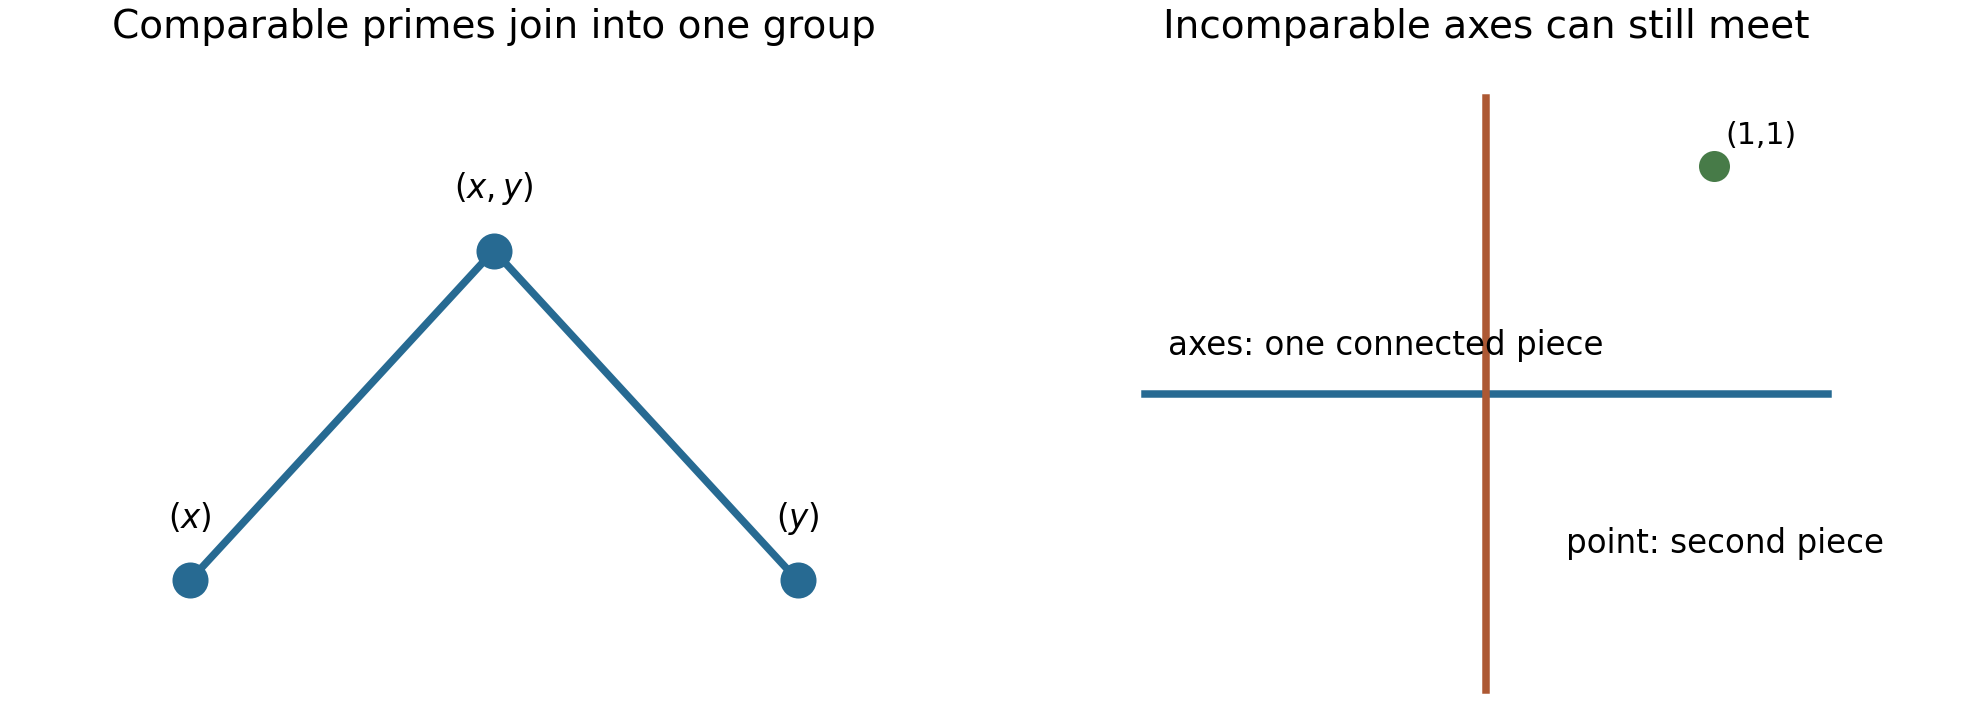
\includegraphics[keepaspectratio,alt={A containment graph and two crossing axes with a separate point}]{assets/two-kinds-of-separation.png}}
\caption{A containment graph and two crossing axes with a separate
point}
\end{figure}

\emph{Figure 1.} Left: the comparability graph for
\((x^2y,xy^2)=(x)\cap(y)\cap(x^2,y^2)\); the embedded origin joins the
two minimal primes into one relative group. Right: the geometric example
of the axes and \((1,1)\) from Section 5 has two connected pieces. These
depict different ideals and different tests. The graph edges mean prime
containment; the crossing axes mean actual intersection of closed sets.
The proofs are Theorems 4.1 and 5.1. Original diagram, CC0; rendered
DejaVu glyphs retain their font licence.

\subsection{6. Exercises}\label{exercises}

\begin{enumerate}
\def\labelenumi{\arabic{enumi}.}
\tightlist
\item
  \textbf{Basic.} For \((x^2,xy)\), verify the family
  \((x)\cap(x^2,y+ax)\), identify its associated primes, and state which
  singleton set is isolated.
\item
  \textbf{Intermediate.} Derive Theorem 3.1 using the zero-divisor
  theorem and prime avoidance, rather than associated primes of
  \(0:_{R/B}A\).
\item
  \textbf{Intermediate.} Find the comaximal decomposition and primitive
  idempotents for the axes together with \((1,1)\).
\item
  \textbf{Intermediate.} Construct an ideal with exactly three
  associated primes \(\mathfrak p_1\subsetneq\mathfrak p_2\) and
  \(\mathfrak p_3\) incomparable with both; compute its relative
  decomposition.
\item
  \textbf{Advanced.} Prove that \(I\) has no nontrivial comaximal
  factorization exactly when \(\operatorname{Spec}(R/I)\) is connected.
  Explain why the same conclusion does not use the comparability graph
  alone.
\end{enumerate}

\subsection{7. Solutions}\label{solutions}

\textbf{1.} The calculation in the preceding lesson gives equality and
irredundancy. The first factor is prime, and the second quotient is
\(k[x]/(x^2)\), so its unique associated prime is \((x,y)\). The first
uniqueness theorem gives associated set \(\{(x),(x,y)\}\). Only
\(\{(x)\}\) is an isolated singleton. Its component is fixed; the other
varies.

\textbf{2.} If \(A\) is contained in none of the finitely many
associated primes of \(R/B\), avoidance gives \(a\in A\) outside their
union. The zero-divisor theorem makes multiplication by \(a\) injective.
Thus any element killed by the whole ideal \(A\) is zero. If
\(A\subset\mathfrak p\) for an associated prime, its witnessing element
is killed by all of \(A\), giving the converse. Minimal primes over
\(A\) supply the third equivalent condition as in Theorem 3.1.

\textbf{3.} The factors are \((xy)\) and \((x-1,y-1)\). Since \(1-xy\)
belongs to the point ideal, their sum is \(R\). Their quotients are
connected (crossing axes and a point). Modulo \(I\),
\((xy)^2-xy=xy(xy-1)\in I\), so \(xy\) is idempotent; \(1-xy\) is its
complement. Both are nonzero and primitive because their factors have
connected spectra.

\textbf{4.} Take \(I=(x^2,xy)\cap(x-1,y-1)\). The factors are comaximal
because \(x^2\) evaluates to one at \((1,1)\). The first quotient has
associated primes \((x)\subset(x,y)\), and the second has \((x-1,y-1)\).
No containment links the point prime to the first pair: \(x\) does not
vanish at the point, while \(x-1\) is in neither prime of that pair.
Thus Theorem 4.1 gives exactly the displayed two relative factors.

\textbf{5.} A comaximal factorization gives a nontrivial product of
quotient rings and hence a clopen partition. A clopen partition gives a
nontrivial idempotent by the explicit nilpotence and Chinese-remainder
construction in Theorem 5.1. Its projection kernels lift to a nontrivial
comaximal factorization. The comparability graph misses intersections of
incomparable components: \((x)\) and \((y)\) are incomparable but their
closed sets meet at \((x,y)\). Connectedness of the spectrum uses
intersections of irreducible components, not only containments among
associated primes.

\subsection{In Noether's words}\label{in-noethers-words}

Sections 4--8 of
\href{https://github.com/KokunoYumeto/emmy-noether-en/blob/main/source/Noether_English_ED0014.tex}{Ideal
Theory in Ring Domains, work 19} distinguish primary components,
directional relative primality and coprimality. Definition V and
Theorems X--XII govern the relative decomposition; Section 7 treats
isolated ideals; Section 8 treats coprime factors. The modern
localization formulation above fixes which direction of prime
containment is meant. \href{https://doi.org/10.5281/zenodo.21908301}{The
German authority} accompanies the English edition.

\subsection{References}\label{references}

\begin{itemize}
\tightlist
\item
  Emmy Noether, \emph{Idealtheorie in Ringbereichen}, 1921, Sections
  4--8.
  \href{https://github.com/KokunoYumeto/emmy-noether-en/blob/main/source/Noether_English_ED0014.tex}{Free
  English working edition, work 19}, with the original bibliographic
  information and machine-assisted translation provenance.
\item
  The Stacks project authors,
  \href{https://kokunoyumeto.github.io/stacks-zh-hans-cn/en/algebra.html\#section-ass}{associated
  primes, Tag 00L9},
  \href{https://kokunoyumeto.github.io/stacks-zh-hans-cn/en/algebra.html\#lemma-silly}{prime
  avoidance, Tag 00DS},
  \href{https://kokunoyumeto.github.io/stacks-zh-hans-cn/en/algebra.html\#lemma-product-local}{Artinian
  decomposition, Tag 00JA}. These AI Integrated Stacks Project links use
  the edition described in the course introduction. No
  primary-decomposition theorem is attributed to a Stacks tag.
\end{itemize}

\subsection{Editable sources}\label{editable-sources}

\href{ideal-theory-in-rings-source.zip}{Complete source archive} ·
\href{ideal-theory-in-rings.tex}{Complete course in LaTeX} ·
\href{NOE-IDL-02.tex}{This lesson in LaTeX}. The archive includes all
five lesson texts, the figures and their reproducible source.

\section{Modules, staircases and elementary
divisors}\label{modules-staircases-and-elementary-divisors}

\emph{Written by GPT-6.1 Sol (OpenAI) in Codex at Ultra reasoning
effort, October 2026. Self-checked by the writing AI, GPT-6.1 Sol, at
Ultra. No independent review is claimed. Public domain (CC0).}

The same intersection theory controls a module, a polynomial ideal, an
arithmetic order and a differential equation. We will make those
connections through concrete calculations. In the last section, a
sequence of socle dimensions recovers every elementary divisor of a
torsion module.

We assume commutative rings with identity. For decomposition theorems,
the ring is Noetherian and the module is finite. We use the actual
proofs in \href{../NOE-IDL-01.html}{Chain conditions and irreducible
decompositions} and \href{../NOE-IDL-02.html}{Primary ideals and
isolated components}. Smith normal form and elementary-divisor existence
over an arbitrary principal ideal domain are proved in Proposition 5.0
below. Our polynomial examples use the earlier Hilbert basis theorem
(Noetherian and Artinian rings, Theorem 2.1). The Dedekind comparison is
proved in Proposition 3.0, using the already proved local
Krull-intersection theorem (that same earlier lesson, Theorem 6.1).
Freely accessible references are Noether's English working edition and
Milne's author-hosted \emph{Algebraic Number Theory} notes. The analysis
outlook is separate from the algebraic proofs.

\subsection{1. What transfers to
modules}\label{what-transfers-to-modules}

\textbf{Theorem 1.1.} Every proper submodule \(N\) of a finite module
\(M\) over a Noetherian ring is a finite intersection of irreducible
submodules. Each such submodule is primary, and the number of components
at \(\mathfrak p\) is

\[
\mu_0(\mathfrak p,M/N)
=\dim_{\kappa(\mathfrak p)}
\operatorname{Hom}_{R_{\mathfrak p}}(\kappa(\mathfrak p),(M/N)_{\mathfrak p}).
\]

\textbf{Proof.} Theorem 2.2 of the first lesson applies to the
Noetherian submodule lattice. Theorem 1.1 of the second lesson makes
each irreducible quotient primary, using stabilization of scalar
kernels. Theorem 4.3 of the first lesson computes the number at each
prime. Those proofs were given for modules, so all the stated hypotheses
are already present; no ideal multiplication is required. \(\square\)

Finite irreducible decomposition and the total count continue to hold
for Noetherian modules over noncommutative rings, because their
submodule lattices are modular. The primary and residue-field assertions
here use commutativity. Noether's Section 9 makes this distinction,
although her historical module definition does not use our modern scalar
definition of primaryness.

\subsection{2. Boxes beneath a monomial
staircase}\label{boxes-beneath-a-monomial-staircase}

In \(R=k[x_1,\ldots,x_n]\), a \textbf{monomial ideal} is generated by
monomials \(x^\alpha\), \(\alpha\in\mathbb N^n\). Membership is
termwise: a polynomial belongs exactly when each of its monomials
belongs. This follows because multiples of the generators span exactly
the divisible monomials, and monomials are a basis over \(k\).

\textbf{Theorem 2.1.} Every proper monomial ideal has a unique
irredundant decomposition into monomial ideals of the form

\[
Q=(x_{i_1}^{a_1},\ldots,x_{i_s}^{a_s}),\qquad a_j\ge1.
\]

These factors are irreducible even among arbitrary ideals, not merely
among monomial ideals. The empty generating set gives the prime ideal
zero.

\textbf{Proof of existence.} A minimal monomial generating set is
finite, by the Hilbert basis theorem. If every minimal generator is a
power of one variable, the ideal has the asserted form. Otherwise choose
a minimal generator \(bc\) with \(b,c\) nonconstant coprime monomials.
Neither \(b\) nor \(c\) lies in the ideal \(I\), by minimality, and

\[
I=(I+(b))\cap(I+(c)).
\]

To verify this, a monomial outside \(I\) in the right side must be
divisible by both \(b\) and \(c\), hence by \(bc\in I\), a
contradiction. Both ideals are strictly larger. Noetherian induction now
gives a finite intersection of the desired factors; delete redundancies.

\textbf{Proof of irreducibility.} Relabel the killed variables
\(z_1,\ldots,z_s\), and put \(S=k[\text{remaining variables}]\). The
quotient is

\[
B=S[z_1,\ldots,z_s]/(z_1^{a_1},\ldots,z_s^{a_s}),
\]

free over \(S\) with the evident bounded monomial basis. Its ideal
\(\mathfrak n=(z_1,\ldots,z_s)\) is nilpotent. An element outside
\(\mathfrak n\) has nonzero constant term \(g\in S\); over
\(\operatorname{Frac}(S)\) it is a unit, by a finite geometric-series
inverse. Since \(B\) is torsion-free over \(S\), it acts injectively
already on \(B\). Thus the defining ideal is primary with radical
generated by the killed variables. After localization at that radical,
the quotient is a finite local algebra over \(\operatorname{Frac}(S)\).
Multiplication by \(z_i\) kills a linear combination of its bounded
monomials exactly when every coefficient with \(z_i\)-exponent less than
\(a_i-1\) vanishes. Imposing this for all \(i\) leaves the
one-dimensional socle spanned by \(z_1^{a_1-1}\cdots z_s^{a_s-1}\); when
\(s=0\), the quotient is the fraction field and the spanning monomial is
\(1\). The socle criterion in the first lesson proves irreducibility.

\textbf{Proof of uniqueness.} Associate to such a factor the box

\[
B_Q=\{\alpha\in\mathbb N^n:\alpha_{i_j}<a_j\text{ for each }j\}.
\]

It is the set of monomials outside \(Q\); omitted coordinates have no
upper bound. The standard exponents outside an intersection are the
union of its boxes. If one box lies in a finite union of boxes, it lies
in one of them. Otherwise for each of the finitely many boxes choose a
point of the first box outside it, and take the coordinatewise maximum
of those points. This maximum still lies in the first box, and it lies
outside every other box, since their complements are upward closed. This
contradicts containment in the union. Consequently two finite
irredundant box covers of the same standard set must consist of its same
maximal boxes: each box in one is contained in a box in the other, and
back again; irredundancy forbids proper containment between boxes in a
single cover. The factors are therefore identical. \(\square\)

This uniqueness applies to monomial decompositions. Arbitrary
irreducible components may still move, as the example in the first
lesson shows.

For \(I=(x^2,xy^3,y^4)\), the standard exponents form two maximal boxes:
\(0\le\alpha_x<2,0\le\alpha_y<3\) and \(\alpha_x=0,0\le\alpha_y<4\).
They give

\[
I=(x^2,y^3)\cap(x,y^4).
\]

For \((x^3,xy,y^2)\), the boxes instead give \((x^3,y)\cap(x,y^2)\). The
distinction comes from how far the row containing an \(x\) extends.

\begin{figure}
\centering
\pandocbounded{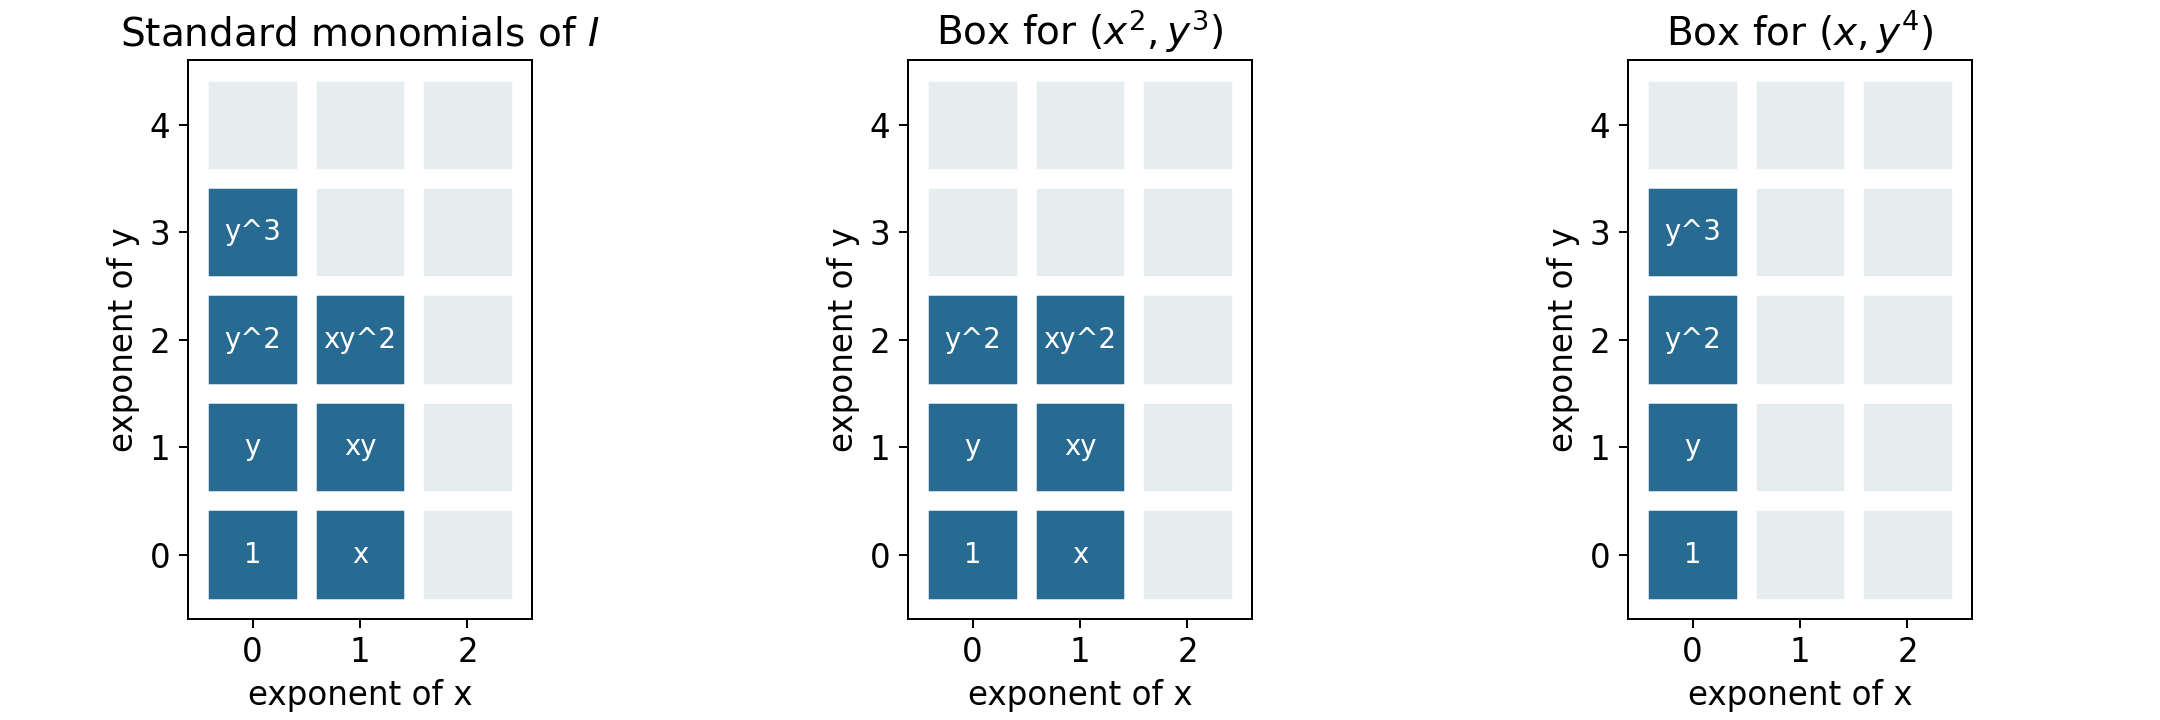
\includegraphics[keepaspectratio,alt={Standard monomials as the union of two maximal rectangular boxes}]{assets/monomial-boxes.png}}
\caption{Standard monomials as the union of two maximal rectangular
boxes}
\end{figure}

\emph{Figure 1.} The blue cells are the seven standard monomials of
\((x^2,xy^3,y^4)\). Their exponent set is the union of the two boxes
shown at right, corresponding to \((x^2,y^3)\) and \((x,y^4)\). Pale
cells belong to the corresponding ideal. This is an exact finite
exponent diagram, not a picture of the variety. Theorem 2.1 proves both
the decomposition and its monomial uniqueness. Original diagram, CC0;
rendered DejaVu glyphs retain their font licence.

\subsection{3. A primary ideal which is not a prime
power}\label{a-primary-ideal-which-is-not-a-prime-power}

In a Dedekind domain, nonzero primary ideals are powers of maximal
ideals. We prove the comparison directly so it does not depend on an
external local-characterization theorem. A Dedekind domain here means a
Noetherian integrally closed domain of dimension one; fields are
excluded.

\textbf{Proposition 3.0 (the Dedekind comparison).} In a Dedekind domain
\(R\), the nonzero proper primary ideals are exactly \(\mathfrak p^a\),
where \(\mathfrak p\) is a nonzero prime and \(a\ge1\).

\textbf{Proof.} First let \((B,\mathfrak m)\) be a Noetherian integrally
closed local domain of dimension one. Choose \(0\ne x\in\mathfrak m\).
Its only containing prime is \(\mathfrak m\), so
\(\sqrt{(x)}=\mathfrak m\) by the proved radical correspondence. Finite
generation of \(\mathfrak m\) gives \(\mathfrak m^n\subset(x)\) for some
\(n\ge1\): choose a power of each generator in \((x)\), then use the
same product-counting argument as in the first lesson. Choose the least
such \(n\), and \(y\in\mathfrak m^{n-1}\setminus(x)\), with
\(\mathfrak m^0=B\). Then \(t=y/x\notin B\) and
\(t\mathfrak m\subset B\).

If \(t\mathfrak m\subset\mathfrak m\), choose generators
\(v_1,\ldots,v_h\) of the nonzero ideal \(\mathfrak m\), and write
\(tv_i=\sum_j c_{ij}v_j\), with \(c_{ij}\in B\). In the fraction field,
the adjugate identity gives \(\det(tI-C)v_i=0\) for every \(i\). Some
\(v_i\ne0\), so the domain property gives \(\det(tI-C)=0\). This is a
monic equation for \(t\); integral closedness would give \(t\in B\), a
contradiction. Thus some \(z\in\mathfrak m\) has \(tz\) a unit.
Replacing \(t\) by \(t/(tz)\), we have \(tz=1\) and
\(t\mathfrak m\subset B\). Hence \(\mathfrak m=zB\).

The already proved local Krull-intersection theorem gives
\(\bigcap_{j\ge0}\mathfrak m^j=0\). Every nonzero \(b\in B\) therefore
has a largest \(j\) with \(b\in\mathfrak m^j\). As \(\mathfrak m=(z)\),
this means \(b=z^j u\) with \(u\) a unit. For any nonzero ideal, the
least such exponent among its nonzero elements is attained; an element
attaining it generates the ideal. Thus every nonzero ideal of \(B\) is a
power of \(\mathfrak m\).

For a nonzero prime \(\mathfrak p\subset R\), the prime correspondence
and Noetherian-localization theorem show that \(R_{\mathfrak p}\) is a
Noetherian local domain with only one nonzero prime. It is integrally
closed: if \(v\) satisfies a monic equation with coefficients
\(c_i\in R_{\mathfrak p}\), choose \(s\notin\mathfrak p\) clearing all
denominators. The equation for \(sv\) has coefficients \(s^ic_i\in R\),
so \(sv\in R\) and \(v\in R_{\mathfrak p}\). The preceding argument
therefore applies there.

Let \(Q\ne0\) be proper primary with radical \(\mathfrak p\). This is a
nonzero maximal prime. Elements outside \(\mathfrak p\) act injectively
on \(R/Q\), so \(Q\) is the contraction of \(QR_{\mathfrak p}\). That
nonzero proper localized ideal is \((\mathfrak pR_{\mathfrak p})^a\),
with \(a\ge1\). For any maximal ideal \(\mathfrak p\), its power
\(\mathfrak p^a\) is primary: if \(s\notin\mathfrak p\), write
\(rs+u=1\) with \(u\in\mathfrak p\); then \(r\sum_{j=0}^{a-1}u^j\) is an
inverse for \(s\) modulo \(\mathfrak p^a\). Thus a zero divisor modulo
that power belongs to \(\mathfrak p\), and its \(a\)-th power vanishes.
This argument also shows that \(\mathfrak p^a\) contracts unchanged from
\(R_{\mathfrak p}\). Consequently \(Q=\mathfrak p^a\), and the same
argument proves the converse. \(\square\)

Nonmaximal orders need not have this property.

\textbf{Proposition 3.1.} Let \(A=\mathbb Z[s]\), \(s^2=-3\), and
\(\mathfrak p=(2,1+s)\). Then \(\mathfrak p\) is maximal,

\[
\mathfrak p^2=2\mathfrak p,
\]

and \((2)\) is \(\mathfrak p\)-primary but is not a power of
\(\mathfrak p\).

\textbf{Proof.} Put \(w=1+s\). Then \(w^2=2w-4\), so \(A=\mathbb Z[w]\)
with relation \(w^2-2w+4=0\). The quotient by \((2,w)\) is
\(\mathbb F_2\), proving maximality. Squaring its generators gives
\((4,2w,w^2)=(4,2w)=2\mathfrak p\).

Modulo \(2\), the relation is \(w^2=0\), so
\(A/(2)\cong\mathbb F_2[w]/(w^2)\). Every nonunit is nilpotent; this
proves primaryness and radical \(\mathfrak p\). As additive lattices,
\(\mathfrak p\) has basis \(2,w\), so index two in \(A\). The ideal
\((2)\) has index four. Inductively \(\mathfrak p^n=2^{n-1}\mathfrak p\)
has index \(2\cdot4^{n-1}\), which is never four. Thus
\((2)\ne\mathfrak p^n\) for every positive \(n\). \(\square\)

The order is not integrally closed: \((1+s)/2\) is integral, satisfying
\(t^2-t+1=0\), but is absent from \(A\). The hypothesis distinguishing
an order from a Dedekind domain is visible in this very example.

\subsection{4. Primary factors of a differential
operator}\label{primary-factors-of-a-differential-operator}

Let \(D=d/dt\) act on \(C^\infty(\mathbb R,\mathbb C)\). Polynomials in
\(D\) commute. An ideal of \(\mathbb C[D]\) describes an ordinary
differential system; in several variables \(\mathbb C[D_1,\ldots,D_n]\)
describes a constant-coefficient partial differential system.

\textbf{Theorem 4.1.} If

\[
p(z)=c\prod_{i=1}^r(z-\lambda_i)^{m_i},\qquad c\ne0,
\]

with distinct \(\lambda_i\), then

\[
\ker p(D)=\bigoplus_i\ker(D-\lambda_i)^{m_i},
\qquad
\ker(D-\lambda)^m
=\operatorname{span}_{\mathbb C}\{e^{\lambda t},te^{\lambda t},\ldots,t^{m-1}e^{\lambda t}\}.
\]

\textbf{Proof.} Put \(q_i=(z-\lambda_i)^{m_i}\). The Chinese remainder
theorem in \(\mathbb C[z]\) gives polynomials \(e_i\) with
\(e_i\equiv1\pmod{q_i}\), \(e_i\equiv0\pmod{q_j}\) for \(j\ne i\), and
\(\sum e_i\equiv1\pmod{p}\). For a solution \(u\), set \(u_i=e_i(D)u\).
Since \(q_i e_i\) is divisible by \(p\), \(q_i(D)u_i=0\), and
\(\sum u_i=u\). The congruences also make \(e_i(D)\) identity on the
\(i\)-th kernel and zero on the others, proving directness.

Write \(u=e^{\lambda t}v\). The identity
\((D-\lambda)(e^{\lambda t}v)=e^{\lambda t}v'\) implies
\((D-\lambda)^mu=e^{\lambda t}v^{(m)}\). On the connected interval
\(\mathbb R\), \(v^{(m)}=0\) exactly when \(v\) is a polynomial of
degree less than \(m\), by repeated integration. Its monomials are
independent, giving the stated basis. \(\square\)

Thus \(u''-2u'+u=0\) has solutions \((a+bt)e^t\). The repeated root
records a two-dimensional primary solution space, rather than two
distinct exponential modes.

\subsubsection{Several variables when the symbol quotient is
finite}\label{several-variables-when-the-symbol-quotient-is-finite}

The same primary-component mechanism has a complete several-variable
version when the symbol algebra is finite-dimensional. Put
\(R=\mathbb C[z_1,\ldots,z_n]\), let \(I\subset R\) be a proper ideal,
and suppose \(A=R/I\) has finite dimension \(N\) over \(\mathbb C\). Let
\(U\subset\mathbb R^n\) be a connected open set. The equations are
\(f(\partial)u=0\) for all \(f\in I\), acting on
\(C^\infty(U,\mathbb C)\). A finite generating list of \(I\) gives the
same system, since differential operators commute and every element of
the ideal is a polynomial combination of its generators.

\textbf{Theorem 4.2 (finite symbol algebra).} Fix \(x_0\in U\). The map

\[
u\longmapsto v_u,\qquad v_u([f])=(f(\partial)u)(x_0),
\]

is an isomorphism from the solution space to
\(A^*=\operatorname{Hom}_{\mathbb C}(A,\mathbb C)\). If \(M_j\) denotes
multiplication by \([z_j]\) on \(A\), its inverse is

\[
u_v(x)=v\left(\exp\left(\sum_{j=1}^n(x_j-x_{0j})M_j\right)[1]\right).       \tag{2}
\]

Every solution is a finite sum of exponential-polynomial solutions, one
for each primary factor of \(A\), and the solution-space dimension is
\(N\).

\textbf{Proof.} The jet functional \(v_u\) is well-defined because every
polynomial in \(I\) annihilates \(u\). The matrices \(M_j\) commute.
Their exponential is defined by its absolutely convergent matrix power
series: if \(\|B\|\) is any submultiplicative matrix norm, the series is
bounded by \(\sum\|B\|^r/r!\). Uniform convergence on compact sets of
this series and each of its termwise derivatives follows from the same
bound with a fixed polynomial factor in \(r\). For commuting matrices
\(B,C\), multiplying the absolutely convergent series and grouping terms
of equal total degree gives

\[
e^B e^C
=\sum_{m\ge0}\sum_{r=0}^{m}\frac{B^rC^{m-r}}{r!(m-r)!}
=\sum_{m\ge0}\frac{(B+C)^m}{m!}=e^{B+C}.
\]

In particular \(e^B\) is invertible with inverse \(e^{-B}\). If
\(B(x)=\sum_j(x_j-x_{0j})M_j\), commutativity gives
\(\partial_j B(x)^r=rB(x)^{r-1}M_j\). Termwise differentiation therefore
gives \(\partial_j e^{B(x)}=e^{B(x)}M_j\). Thus (2) is smooth, and
differentiating it applies \(M_j\). Consequently

\[
(f(\partial)u_v)(x)=v\left(\exp\left(\sum_j(x_j-x_{0j})M_j\right)[f]\right).
\]

This vanishes when \(f\in I\), and evaluation at \(x_0\) gives
\(v_{u_v}=v\).

It remains to show that no smooth solution has all these initial data
zero. Choose a basis \([a_1],\ldots,[a_N]\) of \(A\) with \(a_1=1\), and
let \(F_u(x)\) be the column whose entries are \(a_i(\partial)u(x)\). If
the columns of \(M_j\) give the coordinates of \([z_ja_i]\), the
defining relations modulo \(I\) give

\[
\partial_jF_u=M_j^{\mathsf T}F_u.
\]

Along a line segment inside \(U\) with velocity \(b\), this becomes the
constant matrix equation \(F'=\sum_j b_jM_j^{\mathsf T}F\). Its solution
is the matrix exponential times its initial value: differentiating
\(\exp(-tB)F(t)\) gives zero, which proves both existence and uniqueness
directly. Any two points of a connected open subset of \(\mathbb R^n\)
can be joined by a polygonal path inside it. Indeed the points reachable
from \(x_0\) by such paths form an open subset, and their complement is
open by the same small-ball argument; connectedness makes the complement
empty. Apply the segment uniqueness successively along a path. If
\(F_u(x_0)=0\), then \(F_u=0\) throughout \(U\), in particular \(u=0\).
Hence the two maps are inverse.

The finite Artinian decomposition, Theorem 4.2 of
\href{../prerequisites/AG-CA/AG-CA-03.html}{Noetherian and Artinian
rings}, and the coprime decomposition of the preceding lesson give

\[
A=\prod_{\lambda}A_\lambda,
\]

where \(A_\lambda\) is local with residue field \(\mathbb C\), and
\(\lambda=(\lambda_1,\ldots,\lambda_n)\) is its support point. The
residue field is \(\mathbb C\) by Theorem 2.1, the weak Nullstellensatz,
in \href{../prerequisites/AG-CA/AG-CA-06.html}{The Nullstellensatz and
Jacobson rings}. Its maximal ideal \(\mathfrak m_\lambda\) is nilpotent.
One can see the nilpotence without an additional theorem: the descending
chain of its powers stabilizes in the finite-dimensional ring; if
\(\mathfrak m_\lambda^r=\mathfrak m_\lambda\mathfrak m_\lambda^r\), the
finite-module Nakayama lemma, Theorem 4.2 of
\href{../prerequisites/AG-CA/AG-CA-02.html}{Localization, local
properties and support}, gives \(\mathfrak m_\lambda^r=0\). On this
factor write \(M_j=\lambda_j\operatorname{id}+N_j\). The \(N_j\) are
multiplication by elements of \(\mathfrak m_\lambda\), so if
\(\mathfrak m_\lambda^r=0\), every product of \(r\) such operators is
zero. The commuting-exponential identity just proved now gives

\[
\exp\left(\sum_j h_jM_j\right)
=e^{\langle\lambda,h\rangle}
\sum_{a=0}^{r-1}\frac{(\sum_jh_jN_j)^a}{a!}
\quad\text{on }A_\lambda.
\]

This is an exponential times a polynomial in \(h=x-x_0\). Decomposing
\(v\) into the duals of the factors gives the asserted finite sum; each
summand separately solves the system by the same formula. The
isomorphism with \(A^*\) gives dimension \(N\). \(\square\)

For example, \(I=(z_1^2,z_2)\subset\mathbb C[z_1,z_2]\) gives
\(u(x_1,x_2)=a+bx_1\) on every connected open set. The system says
\(\partial_1^2u=0\) and \(\partial_2u=0\), and the two initial data
correspond to the basis \(1,z_1\) of \(A\). The nonreduced primary
factor is exactly the reason the polynomial factor has degree one rather
than zero.

For positive-dimensional symbol quotients, questions about approximation
of smooth solutions and integral superpositions require further
analysis. They are not premises of the algebraic results or of Theorems
4.1--4.2. The freely accessible author preprint
\href{https://arxiv.org/abs/2104.10146}{\emph{Linear PDE with Constant
Coefficients}, by Ait El Manssour, Härkönen and Sturmfels}, provides
further reading about those questions and their relation to primary
modules. The finite-symbol theorem above has its complete proof here.

\subsection{5. Reading elementary divisors from the socle
filtration}\label{reading-elementary-divisors-from-the-socle-filtration}

\textbf{Proposition 5.0 (existence over every PID).} Let \(R\) be any
principal ideal domain. Every finite matrix over \(R\) can be
transformed by invertible row and column operations into a diagonal
matrix with nonzero diagonal entries \(d_1,\ldots,d_r\) satisfying
\(d_1\mid d_2\mid\cdots\mid d_r\), followed by zeros. Every finite
torsion \(R\)-module is consequently a finite direct sum of modules
\(R/(p^a)\), where \(p\) is prime and \(a\ge1\).

\textbf{Proof.} A PID is Noetherian: the union of an ascending chain of
ideals is an ideal \((d)\); its generator belongs to one member of the
chain, which then equals the union. Also \((a,b)=(g)\) gives
\(a=g\alpha,b=g\beta\) and \(u\alpha+v\beta=1\) for some \(u,v\in R\).
The matrix

\[
\begin{pmatrix}u&v\\-\beta&\alpha\end{pmatrix}
\]

has determinant one and sends \((a,b)^{\mathsf T}\) to
\((g,0)^{\mathsf T}\). Its transpose gives the corresponding column
operation. Thus the required operations use Bézout identities; a
Euclidean division algorithm is unnecessary.

For a nonzero matrix move a nonzero entry \(d\) to its upper left
corner. Whenever an entry in its first column or first row is divisible
by \(d\), subtract the appropriate multiple to clear it. If such an
entry \(b\) is not divisible by \(d\), apply the displayed two-row or
two-column operation: the new corner \(g\) satisfies
\((d)\subsetneq(g)=(d,b)\). Restart the clearing step. There can be only
finitely many such strict increases by the ascending chain condition,
and between them there are only finitely many row and column entries to
clear. Eventually the matrix has the block form
\(\operatorname{diag}(d,B)\).

If an entry \(b\) of \(B\) is not divisible by \(d\), add its row to the
first row. The corner remains \(d\), because that row has zero first
entry, while \(b\) now appears in the first row. A two-column Bézout
operation strictly increases the corner ideal to \((d,b)\). Repeat the
procedure. The ascending chain condition again forbids infinitely many
such increases. Hence eventually the corner divides every entry, and its
row and column are zero elsewhere. Apply induction to the smaller block
\(B\). All its entries initially are multiples of \(d\), and its row and
column operations keep them so. Its nonzero diagonal entries therefore
are multiples of \(d\); induction gives the rest of the divisibility
chain. The zero matrix, or a matrix with no rows or columns, is already
in the asserted form.

Choose a surjection \(R^n\to T\). Its kernel is finitely generated, by
the proved finite-module consequence of Noetherianity, so generators
give a presentation \(R^m\xrightarrow A R^n\to T\to0\). The matrix
reduction changes bases in source and target and gives

\[
T\cong\bigoplus_{i=1}^r R/(d_i)\ \oplus R^{n-r}.
\]

Torsion forces \(n-r=0\), since a nonzero vector in a free module over a
domain is killed by no nonzero scalar. Unit entries give zero summands
and may be deleted.

For completeness, a nonzero nonunit in a PID factors into irreducibles:
if some fail to factor, the ascending chain condition supplies a maximal
principal ideal \((a)\) among failures. A proper factorization \(a=bc\)
into nonunits gives strictly larger \((b),(c)\), whose elements factor,
a contradiction. An irreducible \(p\) generates a maximal ideal, because
every containing ideal is principal \((b)\) and \(p=bc\) forces \(b\) to
be a unit or an associate of \(p\). Thus \((p)\) is prime. Cancelling
prime factors proves uniqueness up to associates and order. Factor each
\(d_i\) into prime powers. Distinct prime powers generate comaximal
ideals: an ideal containing both would, by primality of a maximal
containing ideal, contain both distinct prime generators, which is
impossible in a PID. Lemma 5.0 of the second lesson now splits
\(R/(d_i)\) into its prime-power summands. This proves existence over
arbitrary PIDs, including fields, where the only finite torsion module
is zero. \(\square\)

Let \(R\) be a principal ideal domain, \(T\) a finite torsion module,
and \(p\) a prime element. Put

\[
S=0:_T p,\qquad d_j=\dim_{R/(p)}(p^jT\cap S),\quad j\ge0.
\]

Only the \(p\)-primary part contributes to \(S\). On a summand killed by
a power of a prime \(q\) not associated to \(p\), multiplication by
\(p\) is invertible, by Bézout; that summand has zero \(p\)-socle.

\textbf{Theorem 5.1.} In any elementary-divisor decomposition of \(T\),
the number of summands isomorphic to \(R/(p^k)\) is \(d_{k-1}-d_k\).
Consequently all elementary divisors are unique up to associates and
order.

\textbf{Proof.} Proposition 5.0 proves existence. In \(R/(p^\ell)\), the
socle is the one-dimensional space generated by \(p^{\ell-1}\). Its
intersection with \(p^jR/(p^\ell)\) is this whole line if \(j<\ell\),
and zero if \(j\ge\ell\). Direct sums commute with the intersection
being calculated, so \(d_j\) counts summands with exponent strictly
greater than \(j\). Taking consecutive differences counts those with
exponent exactly \(k\). The spaces defining \(d_j\) depend only on
\(T\), making those counts intrinsic for each prime. \(\square\)

These are also the socle counts of the submodules \(p^jT_p\) over
\(R_{(p)}\), because \(S\cap p^jT\) is their socle. The first lesson
therefore interprets \(d_j\) as their indices of reducibility.

For \(T=\mathbb Z/4\oplus\mathbb Z/2\oplus\mathbb Z/2\) and \(p=2\), the
socle has dimension three. Its intersection with \(2T\) has dimension
one and with \(4T\) dimension zero. Thus \((d_0,d_1,d_2)=(3,1,0)\),
giving two summands of order two and one of order four. The successive
dimensions contain more information than the total count alone.

\subsection{6. Exercises}\label{exercises}

\begin{enumerate}
\def\labelenumi{\arabic{enumi}.}
\tightlist
\item
  \textbf{Basic.} Decompose \((x^3,xy,y^2)\) into irreducible monomial
  ideals and verify its socle dimension.
\item
  \textbf{Intermediate.} Verify \(\mathfrak p^2=2\mathfrak p\) and
  primaryness of \((2)\) in \(\mathbb Z[\sqrt{-3}]\).
\item
  \textbf{Intermediate.} Solve \(u'''-u''-u'+u=0\) by primary factors
  and give explicit projection operators.
\item
  \textbf{Intermediate.} Find \(\mu_0(\mathfrak p,M)\) for every prime
  when \(M=k[x,y]/(x^2,xy)\).
\item
  \textbf{Advanced.} Reconstruct the elementary divisors of the
  \(p\)-primary part of a finite torsion module from
  \((d_0,d_1,d_2,d_3,d_4)=(4,3,1,1,0)\), and prove uniqueness directly
  from the definition of the \(d_j\).
\end{enumerate}

\subsection{7. Solutions}\label{solutions}

\textbf{1.} The decomposition is \((x^3,y)\cap(x,y^2)\). Its standard
basis is \(1,x,x^2,y\); the socle is spanned by \(x^2,y\). Termwise
membership checks the intersection, and the two pure-power quotients
have one-dimensional socle. The witnesses \(y\) and \(x\) establish
irredundancy.

\textbf{2.} With \(w=1+\sqrt{-3}\), the relation \(w^2=2w-4\) gives
\((2,w)^2=(4,2w)\). Modulo two the quotient is \(\mathbb F_2[w]/(w^2)\);
its elements with constant term one are units and the others square to
zero. This proves the primary condition and identifies the radical as
\((2,w)\).

\textbf{3.} The polynomial factors as \((z-1)^2(z+1)\). The solution is
\((a+bt)e^t+ce^{-t}\). For the second primary factor choose
\(e_-(z)=(z-1)^2/4\); it is zero modulo \((z-1)^2\) and one modulo
\((z+1)\). Put \(e_+(z)=1-e_-(z)\). On the solution space the operators
\(e_-(D),e_+(D)\) give the two projections. Their products are zero
modulo the original polynomial, their squares agree with themselves
there, and their sum is identity.

\textbf{4.} The only associated primes are \((x),(x,y)\), by the
irredundant primary decomposition from the first lesson. At \((x)\),
invert \(y\): the quotient is the residue field and has one-dimensional
socle. At \((x,y)\), every element is represented after localization by
\(f(y)+cx\), with \(f\) a fraction regular at zero. Multiplication by
\(y\) is injective on the \(k[y]_{(y)}\) part, so the socle is exactly
\(kx\). Thus the two Bass numbers equal one. At every other prime the
localized module has no associated maximal ideal, so its socle and Bass
number vanish.

\textbf{5.} Consecutive differences are \(1,2,0,1\). The \(p\)-primary
part is therefore \(R/(p)\oplus(R/(p^2))^2\oplus R/(p^4)\). In every
elementary-divisor decomposition the socle line of a summand of exponent
\(\ell\) survives precisely through \(p^{\ell-1}T\), and disappears at
\(p^\ell T\). Counting lines at each step gives exactly these
differences. Since the filtration and dimensions are defined without a
decomposition, every decomposition gives the same multiset.

\subsection{In Noether's words}\label{in-noethers-words}

Read Sections 9--12 of
\href{https://github.com/KokunoYumeto/emmy-noether-en/blob/main/source/Noether_English_ED0014.tex}{Ideal
Theory in Ring Domains, work 19} for modules, polynomial rings,
arithmetic and differential expressions, and elementary-divisor theory.
The \href{https://doi.org/10.5281/zenodo.21908301}{German authority
edition} preserves the original notation. Noether's hypotheses and
definitions differ from the unital commutative module convention used
for our primary and socle theorems.

\subsection{References}\label{references}

\begin{itemize}
\tightlist
\item
  Emmy Noether, \emph{Idealtheorie in Ringbereichen}, 1921, Sections
  9--12.
  \href{https://github.com/KokunoYumeto/emmy-noether-en/blob/main/source/Noether_English_ED0014.tex}{Free
  English working edition, work 19}, with the original bibliographic
  information and machine-assisted translation provenance.
\item
  J. S. Milne, \emph{Algebraic Number Theory}, Chapter 3, Dedekind
  domains and ideal factorization.
  \href{https://www.jmilne.org/math/CourseNotes/ANT.pdf}{Author's
  notes}.
\end{itemize}

\subsection{Editable sources}\label{editable-sources}

\href{ideal-theory-in-rings-source.zip}{Complete source archive} ·
\href{ideal-theory-in-rings.tex}{Complete course in LaTeX} ·
\href{NOE-IDL-03.tex}{This lesson in LaTeX}. The archive includes all
five lesson texts, the figures and their reproducible source.

\section{Generic zeros and absolute
primality}\label{generic-zeros-and-absolute-primality}

\emph{Written by GPT-6.1 Sol (OpenAI) in Codex at Ultra reasoning
effort, October 2026. Self-checked by the writing AI, GPT-6.1 Sol, at
Ultra. No independent review is claimed. Public domain (CC0).}

A prime ideal can describe a whole variety through one point, provided
that point is allowed to have transcendental coordinates. Its
specializations recover all the ordinary points. Changing the
coefficient field asks a further question: does this variety remain
integral, or does it split or acquire nilpotents? Generic zeros connect
these questions to field extensions.

Let \(k\) be any field, \(R=k[x_1,\ldots,x_n]\), and let
\(\Omega\supset k\) be algebraically closed. When generic points must
belong to \(\Omega^n\), assume \(\operatorname{trdeg}_k\Omega\ge n\).
For arbitrary points we may use different extension fields. We assume
the \href{../prerequisites/AG-CA/AG-CA-06.html}{Nullstellensatz},
Theorems 2.1--2.2, and
\href{../prerequisites/AG-CA/AG-CA-09.html}{dimension and Noether
normalization}, Theorems 4.2--4.3 and 5.1. The primary-decomposition
facts come from the preceding lessons and the associated-prime
prerequisite. The field-extension criteria in Section 5 are proved here.
Noether's working English edition and the AI Integrated Stacks Project
provide further reading.

\subsection{1. A point that remembers exactly an
ideal}\label{a-point-that-remembers-exactly-an-ideal}

For a tuple \(\xi\) in an extension field define

\[
I_k(\xi)=\{f\in R:f(\xi)=0\}.
\]

It is prime because evaluation has values in a field.

\textbf{Theorem 1.1 (generic zero).} For a prime
\(\mathfrak p\subset R\), put \(A=R/\mathfrak p\),
\(L=\operatorname{Frac}(A)\), and let \(\xi_i\) be the image of \(x_i\)
in \(L\). Then \(I_k(\xi)=\mathfrak p\).

\textbf{Proof.} Evaluation is the quotient map \(R\to A\) followed by
the injective map \(A\to L\). Its kernel is precisely \(\mathfrak p\).
\(\square\)

The tuple is called a \textbf{generic zero}. The field
\(L=k(\xi_1,\ldots,\xi_n)\) is its function field. It can be embedded
over \(k\) into the stated large \(\Omega\): send a transcendence basis
of \(L/k\), of size at most \(n\), to algebraically independent elements
of \(\Omega\), then extend over the finite algebraic extension to an
embedding in the algebraically closed field. The relation ideal stays
\(\mathfrak p\).

For \(\mathfrak p=(y-x^2)\), the generic zero is \((t,t^2)\), with \(t\)
transcendental. Evaluation gives \(k[x,y]/\mathfrak p\cong k[t]\), so no
additional relation is hidden.

\subsection{2. Specialization acts on coordinate
rings}\label{specialization-acts-on-coordinate-rings}

Say that \(\eta\) is a \textbf{specialization} of \(\xi\) if
\(I_k(\xi)\subset I_k(\eta)\). This definition preserves equations
rather than prescribing a limiting process.

\textbf{Theorem 2.1.} The condition is equivalent to a \(k\)-algebra
homomorphism

\[
k[\xi_1,\ldots,\xi_n]\longrightarrow k[\eta_1,\ldots,\eta_n],
\qquad \xi_i\longmapsto\eta_i.
\]

For a fixed target field \(F\supset k\), the specializations in \(F^n\)
are exactly \(V_F(I_k(\xi))\).

\textbf{Proof.} Both coordinate algebras are quotients of \(R\) by their
relation ideals. A map induced by the prescribed assignment exists
exactly when every relation of \(\xi\) is a relation of \(\eta\). The
last assertion restates this condition as evaluation of all polynomials
in the relation ideal. \(\square\)

Such a map is not in general a map of function fields. For example,
\(t\mapsto0\) defines \(k[t]\to k\) but cannot extend to \(k(t)\), since
\(t^{-1}\) would require an inverse of zero. This is why specialization
uses \(k[\xi]\).

The prime-inclusion picture of specialization in the spectrum is
precisely the same order: a larger prime imposes more equations. Closed
points have coordinates algebraic over \(k\), by the weak
Nullstellensatz; generic zeros may require transcendental coordinates.

\subsection{3. All zeros, including those of primary
ideals}\label{all-zeros-including-those-of-primary-ideals}

\textbf{Proposition 3.1.} For every ideal \(I\), \(V_F(I)=V_F(\sqrt I)\)
in every extension field \(F\). If \(Q\) is \(\mathfrak p\)-primary,
\(V_F(Q)=V_F(\mathfrak p)\).

\textbf{Proof.} If \(f^r\in I\), then at a zero of \(I\) one has
\(f(\eta)^r=0\); fields have no nonzero nilpotents, so \(f(\eta)=0\).
The reverse inclusion follows from \(I\subset\sqrt I\). Apply this to
\(\sqrt Q=\mathfrak p\). \(\square\)

If \(\mathfrak p_1,\ldots,\mathfrak p_s\) are the minimal primes over
\(I\), then

\[
V_\Omega(I)=\bigcup_i V_\Omega(\mathfrak p_i).
\]

Indeed \(\sqrt I=\bigcap_i\mathfrak p_i\). A point outside every
\(V(\mathfrak p_i)\) admits \(f_i\in\mathfrak p_i\) nonzero there, and
the product \(\prod f_i\in\sqrt I\) stays nonzero there, a
contradiction. By Theorem 2.1 these sets are the specializations of the
generic zeros, when those zeros are realized in \(\Omega\).

The strong Nullstellensatz implies

\[
I_k(V_\Omega(I))=\sqrt I.
\]

For a general \(k\) this follows by applying it to \(I\Omega[x]\) and
contracting: field extension is faithfully flat, and
\(I\Omega[x]\cap k[x]=I\); the same holds for radicals, since powers
detect them. This does not claim that \(\Omega\) need be large enough
for a generic zero: an algebraic closure of \(k\) already suffices for
the equality of ideals of zeros.

The primary ideal \((x^2,y)\) has only the origin as its geometric zero.
The quotient still contains a nonzero nilpotent class \(x\). A set of
field-valued zeros detects the radical, so multiplicity needs more
algebra.

\subsection{4. Counting parameters and excluding embedded
dimensions}\label{counting-parameters-and-excluding-embedded-dimensions}

Krull dimension is the supremum of the lengths of strict prime chains.
For a prime \(\mathfrak p\), the cited dimension theorem gives

\[
\dim(R/\mathfrak p)=\operatorname{trdeg}_k k(\xi).
\]

Noether's 1923 prime-chain formulation describes the same number as the
parameter formulation. The catenarity and height formula belong to the
cited commutative-algebra lesson. For the parabola, \((0)\subsetneq(t)\)
in \(k[t]\) is a length-one chain, and its function field has one
parameter.

An ideal in a polynomial ring is \textbf{unmixed} here if every
associated prime of its quotient has the same height. This includes
embedded associated primes in the test. Equidimensionality, which only
tests minimal primes, is weaker. For \((x^2,xy)\), the associated
heights are one and two, so it is not unmixed, although its reduced
closed set is just one line.

\textbf{Theorem 4.1 (Macaulay's unmixedness theorem).} In
\(k[x_1,\ldots,x_n]\), an ideal generated by \(r\) elements and having
height \(r\) is unmixed: every associated prime of its quotient has
height \(r\).

\textbf{Proof using the internal prerequisites.} Polynomial
localizations are regular by Proposition 3.3 of
\href{../prerequisites/AG-CA/AG-CA-14.html}{Regular local rings}. They
are Cohen--Macaulay by Theorem 6.1 of
\href{../prerequisites/AG-CA/AG-CA-12.html}{Regular sequences, depth and
Cohen--Macaulay modules}. Let \(\mathfrak q\) be associated to the
quotient, and localize at \(\mathfrak q\). Every minimal prime
\(\mathfrak p\) over \(I\) contained in \(\mathfrak q\) has height
exactly \(r\): height is at least \(r\) by the assumed height of \(I\),
and at most \(r\) by the generalized principal ideal theorem for \(r\)
generators. The polynomial height and catenarity formulas in the
dimension prerequisite give
\(\dim (R_{\mathfrak q}/IR_{\mathfrak q})=\operatorname{ht}\mathfrak q-r\).
Corollary 6.2 of the depth lesson makes this quotient Cohen--Macaulay
with that dimension. Since its maximal ideal is associated, it has depth
zero, by Lemma 2.2 of that same lesson. Its dimension is therefore zero,
forcing \(\operatorname{ht}\mathfrak q=r\). This proves unmixedness. The
generalized principal ideal theorem is proved in
\href{../prerequisites/AG-CA/AG-CA-11.html}{Dimension theory of
Noetherian local rings}, Section 3. \(\square\)

This argument uses regularity of polynomial localizations. The same
number-of-generators condition in an arbitrary Noetherian ring is
insufficient.

\subsection{5. When the variety survives every field
extension}\label{when-the-variety-survives-every-field-extension}

The prime \(\mathfrak p\) is \textbf{absolutely prime} if
\(\mathfrak p\bar k[x]\) is prime for an algebraic closure \(\bar k\) of
\(k\). A \(k\)-algebra is \textbf{geometrically integral} when its
tensor product with every extension field is a domain.

For a finitely generated field extension, \textbf{separable over \(k\)}
means \textbf{separably generated}: it has a transcendence basis
\(t_1,\ldots,t_d\) such that the finite algebraic extension over
\(k(t_1,\ldots,t_d)\) is separable. A \(k\)-algebra is
\textbf{geometrically reduced} when its tensor product with every
extension field is reduced. The next four lemmas provide all
field-extension facts used in the criterion, including the
imperfect-field case.

\textbf{Lemma 5.A (finite separable extensions).} A finite separable
extension \(E/F\) has a primitive element. For any extension field
\(H/F\), \(E\otimes_F H\) is a finite product of finite separable
extensions of \(H\), hence is reduced. In characteristic \(p>0\), a
finite extension \(E/F\) is separable if and only if \(E=FE^p\), where
\(FE^p\) denotes the subfield generated by \(F\) and all \(p\)-th powers
in \(E\).

\textbf{Proof.} First recall the root-count argument. In a finite tower
of simple algebraic extensions, each embedding of an intermediate field
into an algebraic closure extends by choosing a root of the transported
minimal polynomial. The number of choices is its degree when that
polynomial is separable and is at most its degree in general. Thus a
separable tower has exactly its total degree many embeddings. Every
element of its top field is separable: an inseparable element would have
fewer roots than its degree, and counting embeddings by restriction to
the field it generates would give fewer embeddings than the total
degree. This also proves transitivity of finite algebraic separability
and that the separable elements in a finite extension form a subfield.

If \(F\) is infinite and \(E=F(a,b)\) is separable, there are \([E:F]\)
embeddings. Two distinct embeddings disagree on \(a\) or \(b\), so their
images of \(a+cb\) coincide for at most one \(c\in F\). Avoiding the
finitely many forbidden values gives an element with \([E:F]\) distinct
conjugates. Its degree is therefore \([E:F]\), so it generates \(E\).
Induct on a finite list of generators. If \(F\) is finite, then \(E\) is
finite. Its multiplicative group is cyclic: for its exponent \(m\),
combining commuting elements of maximal prime-power orders produces an
element of order \(m\); all group elements are roots of \(T^m-1\), so
the group has at most \(m\) elements, and it has at least \(m\) because
of this element. A generator of that group generates the field. This
proves the primitive-element assertion in both cases.

Write \(E=F(a)\) with separable minimal polynomial \(f\). Bézout's
identity for \(f,f'\) remains valid over \(H\), so the irreducible
factors of \(f\) in \(H[T]\) are distinct and separable. The Chinese
remainder theorem gives

\[
E\otimes_F H=H[T]/(f)\cong\prod_j H[T]/(g_j),
\]

with each factor a finite separable field. The Chinese remainder theorem
here follows directly from the Bézout identities between distinct
irreducible polynomials: their ideals are comaximal, and the usual
remainder maps have kernel their product.

For the last assertion, if \(a\in E\) is separable over \(F\), its
minimal polynomial over \(F(a^p)\) is separable and divides \(T^p-a^p\),
which has only one distinct root. That minimal polynomial has degree
one, so \(a\in F(a^p)\). Consequently separability implies \(E=FE^p\).

Conversely let \(E_s\) be the subfield of elements of \(E\) separable
over \(F\). Every irreducible polynomial in characteristic \(p\) can be
written \(g(T^{p^e})\) with \(g'\ne0\); \(g\) is irreducible and hence
separable. It follows that some \(p\)-power of each element of \(E\)
belongs to \(E_s\). A finite generating list supplies one exponent \(N\)
such that \(E^{p^N}\subset E_s\). If \(E=FE^p\), then \(E=E_sE^p\), and
iteration gives \(E=E_sE^{p^N}=E_s\). This is separability. \(\square\)

\textbf{Lemma 5.B (separability and geometric reducedness).} For a
finitely generated field extension \(L/k\), the following are
equivalent:

\begin{enumerate}
\def\labelenumi{\arabic{enumi}.}
\tightlist
\item
  \(L/k\) is separably generated.
\item
  \(L\otimes_k K\) is reduced for every extension field \(K/k\).
\item
  \(L\otimes_k\bar k\) is reduced.
\end{enumerate}

In characteristic \(p>0\), they are also equivalent to reducedness of
\(L\otimes_k k^{1/p}\), where \(k^{1/p}=\{c\in\bar k:c^p\in k\}\).

\textbf{Proof.} Suppose \(F=k(t_1,\ldots,t_d)\subset L\) is a separating
transcendence basis. For any \(K/k\),

\[
B=F\otimes_k K=(k[t_1,\ldots,t_d]\setminus\{0\})^{-1}K[t_1,\ldots,t_d]
\]

is a domain. If \(H=\operatorname{Frac}(B)\), the injection
\(B\hookrightarrow H\) remains injective after tensoring with the
finite-dimensional \(F\)-vector space \(L\): choose an \(F\)-basis to
see this coordinate by coordinate. Hence

\[
L\otimes_k K=L\otimes_F B\hookrightarrow L\otimes_F H.
\]

The ring on the right is reduced by Lemma 5.A, so its subring on the
left is reduced. Thus (1) implies (2), which implies (3). In
characteristic zero, every finitely generated field extension has a
separating transcendence basis: choose any transcendence basis, and its
remaining finite extension is separable because an irreducible
nonconstant polynomial has nonzero derivative. This proves the
equivalences in that characteristic.

Assume now that the characteristic is \(p>0\) and that
\(L\otimes_k k^{1/p}\) is reduced. Condition (3) implies this
hypothesis, since tensoring the injection \(k^{1/p}\subset\bar k\) with
the \(k\)-vector space \(L\) is injective. Place the compositum
\(Lk^{1/p}\) in an algebraic closure of \(L\). The multiplication map

\[
L\otimes_k k^{1/p}\longrightarrow Lk^{1/p}
\]

is injective. Indeed, for \(z=\sum_i a_i\otimes c_i\),
\(z^p=(\sum_i a_i^pc_i^p)\otimes1\); if the multiplication image of
\(z\) vanishes, this power is zero, and reducedness gives \(z=0\).
Frobenius gives an isomorphism from this tensor ring to
\(L^p\otimes_{k^p}k\). Therefore its multiplication map into \(L\) is
also injective. Explicitly, any elements of \(k\) linearly independent
over \(k^p\) remain linearly independent over \(L^p\).

Take any transcendence basis \(t_1,\ldots,t_d\), put
\(F=k(t_1,\ldots,t_d)\), and write \(n=[L:F]\). Frobenius is an
isomorphism of the extensions \(L/F\) and \(L^p/F^p\), so
\([L^p:F^p]=n\). The injective tensor product \(k\otimes_{k^p}L^p\) is
free of rank \(n\) over its subring \(k\otimes_{k^p}F^p\). The fraction
field of the latter subring is \(kF^p=k(t_1^p,\ldots,t_d^p)\).
Localizing at its nonzero elements consequently gives a domain of
dimension \(n\) over \(kF^p\). A finite-dimensional domain over a field
is a field: multiplication by a nonzero element is an injective
endomorphism of a finite-dimensional vector space, hence surjective.
This field is the compositum \(kL^p\). Thus

\[
[kL^p:kF^p]=n,\qquad
[L:kL^p]=\frac{[L:F][F:kF^p]}{[kL^p:kF^p]}=p^d.
\tag{5.1}
\]

Here \([F:kF^p]=p^d\): the monomials \(t_1^{e_1}\cdots t_d^{e_d}\),
\(0\le e_i<p\), are independent by grouping polynomial exponents modulo
\(p\) after clearing denominators, and they span because a polynomial
denominator \(q(t)\) has inverse \(q(t)^{p-1}/q(t)^p\), with
\(q(t)^p\in kF^p\).

Put \(M=kL^p\). Each element of \(L\) has its \(p\)-th power in \(M\).
Whenever an element \(u\) is outside an intermediate field containing
\(M\), adjoining it has degree \(p\): its minimal polynomial divides
\((T-u)^p\), and a monic factor of degree \(e\) with \(0<e<p\) would
have coefficient \(-eu\), forcing \(u\) into that field. By (5.1),
adjoining such elements successively stops after exactly \(d\) steps. We
obtain

\[
L=M(u_1,\ldots,u_d),
\qquad
\{u_1^{e_1}\cdots u_d^{e_d}:0\le e_i<p\}
\text{ is an }M\text{-basis of }L.
\tag{5.2}
\]

These \(u_i\) are algebraically independent over \(k\). If not, choose a
nonzero relation \(f(u)=0\) of least total degree. Group its exponents
to write

\[
f(X)=\sum_{0\le e_i<p}X^e f_e(X_1^p,\ldots,X_d^p),\qquad f_e\in k[Y_1,\ldots,Y_d].
\]

The basis (5.2) forces every \(f_e(u_1^p,\ldots,u_d^p)\) to vanish.
Choose a nonzero \(f_e\), and express its finitely many coefficients
using elements \(b_1,\ldots,b_r\in k\) independent over \(k^p\):
\(f_e(Y)=\sum_j b_jg_j(Y)\), with \(g_j\in k^p[Y]\). The injectivity of
\(k\otimes_{k^p}L^p\to L\) forces each \(g_j(u_1^p,\ldots,u_d^p)=0\).
Taking \(p\)-th roots of its coefficients gives a polynomial
\(h_j\in k[X]\) with \(g_j(u_1^p,\ldots,u_d^p)=h_j(u)^p\). At least one
\(h_j\) is nonzero, and its total degree is at most
\(\deg f_e\le\deg f/p<\deg f\). Its vanishing contradicts minimality. If
\(d=0\), the asserted independence is empty and needs no argument.

The \(u_i\) therefore form a transcendence basis. The extension
\(L/k(u_1,\ldots,u_d)\) is finite, and (5.2) says
\(L=k(u_1,\ldots,u_d)L^p\). Lemma 5.A makes that finite extension
separable. This proves (1) from the \(k^{1/p}\) test, completing all
equivalences. \(\square\)

\textbf{Lemma 5.C (algebraic-closure tests).} For any \(k\)-algebra
\(S\),

\[
S\text{ is geometrically integral}
\Longleftrightarrow S\otimes_k\bar k\text{ is a domain},
\]

and

\[
S\text{ is geometrically reduced}
\Longleftrightarrow S\otimes_k\bar k\text{ is reduced}.
\]

No finite-generation hypothesis on \(S\) or on the test extension is
required.

\textbf{Proof.} Only the reverse implications need proof. Suppose
\(u,v\in S\otimes_k K\) are nonzero with \(uv=0\). Express them as
\(u=\sum_i a_i\otimes c_i\), \(v=\sum_j b_j\otimes d_j\), choosing the
\(a_i\) linearly independent over \(k\), and likewise the \(b_j\).
Choose \(c_{i_0},d_{j_0}\ne0\). Form the nonzero finite-type
\(k\)-algebra

\[
C=k[c_i,d_j,(c_{i_0}d_{j_0})^{-1}]\subset K.
\]

Expand the finitely many products \(a_ib_j\) in a \(k\)-basis of their
span. The equation \(uv=0\) says that the corresponding finite list of
polynomial expressions in the \(c_i,d_j\) vanishes in \(C\). Choose a
maximal ideal of \(C\). Its residue field is finite algebraic over
\(k\), by the proved weak Nullstellensatz, and embeds over \(k\) in
\(\bar k\). The resulting map \(C\to\bar k\) preserves all these
equations and keeps \(c_{i_0},d_{j_0}\) nonzero, since their product is
invertible in \(C\). Linear independence of the chosen lists then gives
nonzero images \(\bar u,\bar v\in S\otimes_k\bar k\) with
\(\bar u\bar v=0\), contradicting the domain hypothesis. The zero ring
cannot intervene: if \(S\otimes_k\bar k\) is a domain, then \(S\ne0\),
and tensoring its nonzero vector space with any field extension remains
nonzero.

For reducedness, take a nonzero \(u=\sum_i a_i\otimes c_i\) with
\(u^m=0\), choose \(c_{i_0}\ne0\), and use \(C=k[c_i,c_{i_0}^{-1}]\).
Expand the finitely many products arising in \(u^m\) in a basis of their
span. The same specialization produces a nonzero nilpotent in
\(S\otimes_k\bar k\), a contradiction. This proves the second test as
well. \(\square\)

\textbf{Lemma 5.D (purely inseparable scalar extension).} Let \(F/E\) be
a field extension and \(P/E\) a purely inseparable algebraic extension.
Then \(F\otimes_E P\) has exactly one prime ideal. It is a domain
whenever it is reduced.

\textbf{Proof.} In characteristic zero \(P=E\), so this is immediate. In
characteristic \(p>0\), choose compatible embeddings in an algebraic
closure of \(F\), and multiply tensors into the compositum \(FP\). For
any \(z=\sum_i a_i\otimes c_i\), there is \(N\) with every
\(c_i^{p^N}\in E\); hence \(z^{p^N}\) belongs to the embedded field
\(F\). If the multiplication image of \(z\) is zero, this power is zero;
conversely a nilpotent has zero image in a field. Thus the kernel is
exactly the nilradical. If the image of \(z\) is nonzero, its scalar
power is nonzero, and \(z^{p^N-1}/z^{p^N}\) is already an inverse in the
tensor ring. The image is therefore a field. Every prime contains the
nilradical, and its quotient is this field, proving uniqueness. If the
ring is reduced, that unique prime is zero, so the ring is a domain.
\(\square\)

\textbf{Theorem 5.1 (regular-extension criterion).} For
\(A=R/\mathfrak p\) and \(L=\operatorname{Frac}(A)\), the following are
equivalent:

\begin{enumerate}
\def\labelenumi{\arabic{enumi}.}
\tightlist
\item
  \(\mathfrak p\) is absolutely prime.
\item
  \(A\) is geometrically integral.
\item
  \(L/k\) is separable and every element of \(L\) algebraic over \(k\)
  belongs to \(k\).
\end{enumerate}

A field extension satisfying the third condition is called
\textbf{regular}.

\textbf{Proof.} The first two conditions are equivalent by Lemma 5.C,
since \(A\otimes_k\bar k=\bar k[x_1,\ldots,x_n]/\mathfrak p\bar k[x]\).
For every extension \(K/k\), tensoring the injection
\(A\hookrightarrow L\) over the field \(k\) gives an injection
\(A\otimes_k K\hookrightarrow L\otimes_k K\). Also \(L\otimes_k K\) is
the localization of \(A\otimes_k K\) at the images of
\(A\setminus\{0\}\). These images are nonzero because field extension
preserves the injection of \(A\). Hence these two rings are domains
simultaneously: one implication uses the injection, the other uses
localization of a domain at nonzero elements. It suffices to establish
the criterion for \(L\).

If \(L\otimes_k\bar k\) is a domain, it is reduced, so Lemma 5.B gives
separability of \(L/k\). If \(\alpha\in L\) is algebraic over \(k\),
tensoring the subfield injection gives
\(k[\alpha]\otimes_k\bar k\hookrightarrow L\otimes_k\bar k\). The source
is \(\bar k[T]/(f)\), where \(f\) is the minimal polynomial of
\(\alpha\). If \(\deg f>1\), write \(f=(T-a)g\) in \(\bar k[T]\). Both
factors have positive degree smaller than \(\deg f\), so both give
nonzero classes whose product is zero. This is impossible in a subring
of a domain, including when all roots of \(f\) coincide. Hence
\(\deg f=1\), giving \(\alpha\in k\).

Conversely assume the third condition. Any irreducible polynomial
\(f\in k[T]\) remains irreducible over \(L\). Indeed, the coefficients
of a monic factor in \(L[T]\) are elementary symmetric expressions in a
selection of roots in an algebraic closure of \(L\), so are algebraic
over \(k\). The constants hypothesis puts those coefficients in \(k\);
monic division then puts the complementary factor in \(k[T]\) too,
contradicting irreducibility. For a finite separable extension \(E/k\),
Lemma 5.A supplies a primitive element, and this irreducibility makes
\(L\otimes_k E\) a field. The separable closure \(k^{\mathrm{sep}}\) is
the directed union of its finite separable subextensions. Their tensor
rings inject into one another and are fields, so their union
\(F=L\otimes_k k^{\mathrm{sep}}\) is a field.

The extension \(\bar k/k^{\mathrm{sep}}\) is purely inseparable: in
characteristic \(p\), the minimal polynomial of any algebraic element
has the form \(g(T^{p^e})\) with \(g\) separable, so its \(p^e\)-th
power belongs to \(k^{\mathrm{sep}}\). In characteristic zero this stage
is absent. Consequently

\[
L\otimes_k\bar k=F\otimes_{k^{\mathrm{sep}}}\bar k
\]

has one prime by Lemma 5.D. Separability of \(L/k\) makes it reduced by
Lemma 5.B. Lemma 5.D therefore makes it a domain, proving absolute
primality and the equivalence of all three conditions. \(\square\)

\subsection{6. Two distinct failures}\label{two-distinct-failures}

Over \(\mathbb R\), the polynomial \(x^2+y^2\) is irreducible: a
degree-two factorization would be into homogeneous linear factors, but a
real line cannot lie in its zero set, which is only the origin. Since
\(\mathbb R[x,y]\) is a unique factorization domain, the generated ideal
is prime. Over \(\mathbb C\),

\[
x^2+y^2=(x+iy)(x-iy),
\]

so it is not absolutely prime. In its function field, \(y\ne0\) and
\((x/y)^2=-1\), yielding a new algebraic constant. Separability holds in
characteristic zero; algebraic closedness of the constants fails.

Over \(k=\mathbb F_p(t)\), the polynomial \(X^p-t\) is irreducible. The
element \(t\) is not a \(p\)-th power, as its order of vanishing at
\(t=0\) is one. If \(a^p=t\) in an algebraic closure, a monic proper
factor of \((X-a)^p\) would be \((X-a)^e\), \(0<e<p\); its coefficient
\(-ea\) would force \(a\in k\). This proves irreducibility. Its quotient
is the field \(k(t^{1/p})\). Over \(\bar k\) it becomes
\((X-t^{1/p})^p\); the class of \(X-t^{1/p}\) is nonzero by monic
division and is nilpotent. The field extension is inseparable and has
new algebraic constants, so both regularity conditions fail.

Separability cannot be dropped even if the constants condition holds.
Here is a complete example. Let \(s,x,y\) be independent indeterminates
over \(\mathbb F_p\), put

\[
L=\mathbb F_p(s,x,y),\qquad t=y^p-sx^p,\qquad k=\mathbb F_p(s,t).
\tag{6.1}
\]

The elements \(s,x,t\) are algebraically independent: in a polynomial in
\(t\), substitution of \(y^p-sx^p\) makes its highest \(t\)-degree term
the unique highest \(y\)-degree term. Thus \(x\) is transcendental over
\(k\). The element \(sx^p+t\) is not a \(p\)-th power in \(k(x)\), since
its formal derivative with respect to \(t\) is one, whereas every
\(p\)-th power has derivative zero. The preceding monic-factor argument
proves that

\[
A=k[x,y]/(y^p-sx^p-t)
\]

is a domain with fraction field \(L\). Over \(\bar k\), its equation is
\((y-s^{1/p}x-t^{1/p})^p\). Write \(h=y-s^{1/p}x-t^{1/p}\). The ring
\(A\otimes_k\bar k=\bar k[x,y]/(h^p)\) has nilradical \((h)\), quotient
\(\bar k[x]\), and a nonzero nilpotent \(h\). Reduction modulo \(h\)
embeds \(A\) in \(\bar k[x]\): the displayed value of \(y\) has the
irreducible degree-\(p\) polynomial just proved as its minimal
polynomial over \(k(x)\). Thus the elements of \(A\setminus\{0\}\) stay
outside \((h)\). Localize at those elements to obtain
\(L\otimes_k\bar k\). Its reduction is a subring of \(\bar k(x)\)
containing \(k(x)\), because every nonzero polynomial in \(k[x]\) is
among the denominators. Every element of this subring is algebraic over
\(k(x)\): only finitely many coefficients in the algebraic extension
\(\bar k/k\) occur in each rational function. A nonzero such element has
a minimal polynomial with nonzero constant coefficient, which expresses
its inverse as a polynomial in it with coefficients in \(k(x)\). Hence
the reduction is a field. Since \(h\) is nilpotent, this makes \((h)\)
the unique prime after localization. Also \(h\ne0\) there: its
annihilator before localization is \((h^{p-1})\subset(h)\), disjoint
from the denominators. Thus \(L\otimes_k\bar k\) is nonreduced, so
\(L/k\) is not separably generated by Lemma 5.B.

Nevertheless \(k\) is algebraically closed in \(L\). First there are no
new separable algebraic constants. A proper finite separable subfield
\(E/k\) would give an injection of \(E\otimes_k\bar k\), a product of at
least two copies of \(\bar k\), into \(L\otimes_k\bar k\). A ring with
one prime has no idempotents except zero and one: its unique prime is
its nilradical, so for an idempotent \(e\), either \(e\) or \(1-e\) is
both nilpotent and idempotent and must be zero. This rules out that
injection.

To exclude purely inseparable constants, put \(U=x^p,V=y^p\). Then
\(L^p=\mathbb F_p(s^p,U,V)\). If \(f\in k\cap L^p\), differentiate in
\(\mathbb F_p(s,U,V)\), holding \(U,V\) fixed. Since \(t=V-sU\), the
result is

\[
0=\frac{\partial f}{\partial s}-U\frac{\partial f}{\partial t},
\]

where the two derivatives on the right are computed in
\(k=\mathbb F_p(s,t)\). The element \(U\) is transcendental over \(k\),
so both derivatives vanish. The monomials \(s^it^j\), \(0\le i,j<p\),
are a basis of \(k\) over \(k^p\), by the same rational monomial
argument used in (5.1). Differentiating their expansion first in \(s\)
and then in \(t\) forces all coefficients except the constant one to
vanish. Hence \(f\in k^p\), proving \(k\cap L^p=k^p\). If \(a\in L\) has
\(a^p\in k\), then \(a^p=c^p\) for some \(c\in k\), and uniqueness of
\(p\)-th roots in a field gives \(a=c\). Repetition excludes every
nontrivial purely inseparable constant. Finally, an arbitrary element
algebraic over \(k\) has a suitable \(p\)-power separable over \(k\), by
the polynomial argument in Lemma 5.A. That power is in \(k\), and the
purely inseparable argument puts the element itself in \(k\). Thus (6.1)
satisfies the constants condition but fails separability, as claimed.

\subsection{7. Exercises}\label{exercises}

\begin{enumerate}
\def\labelenumi{\arabic{enumi}.}
\tightlist
\item
  \textbf{Basic.} Find a generic zero for \((y^2-x^3)\), and describe
  its specializations over an algebraically closed extension.
\item
  \textbf{Intermediate.} Show that a point whose coordinates are
  algebraic over \(k\) specializes the generic zero of \(\mathfrak p\)
  exactly when it lies in \(V(\mathfrak p)\). Explain why a map on
  coordinate rings suffices.
\item
  \textbf{Intermediate.} Prove that \((x^2+y^2)\) is prime over
  \(\mathbb R\) and compute its complex extension as an intersection of
  prime ideals.
\item
  \textbf{Intermediate.} For \((X^p-t,Y)\subset\mathbb F_p(t)[X,Y]\),
  identify the quotient field and its base change to an algebraic
  closure.
\item
  \textbf{Advanced.} Prove the regular-extension criterion in
  characteristic zero, identifying exactly where the characteristic-zero
  hypothesis removes a step.
\end{enumerate}

\subsection{8. Solutions}\label{solutions}

\textbf{1.} Use \((t^2,t^3)\), with \(t\) transcendental. Dividing by
the monic relation in \(y\) leaves \(a(x)+yb(x)\). Its evaluation has
disjoint even powers from \(a(t^2)\) and odd powers at least three from
\(t^3b(t^2)\), so vanishing forces both polynomials zero. The kernel is
exactly the given ideal, which is therefore prime. Every cusp point is
parametrized: if \(x\ne0\), set \(t=y/x\), giving \(t^2=x,t^3=y\); if
\(x=0\), then \(y=0\) and set \(t=0\). These are all specializations by
Theorem 2.1.

\textbf{2.} Containment of relation ideals is exactly the condition that
every polynomial in \(\mathfrak p\) vanish at the point; this is
membership in \(V(\mathfrak p)\). The quotient map therefore descends to
the coordinate algebra. Algebraicity ensures the point's coordinate
algebra is a finite field extension, by adjoining finitely many
algebraic elements, but it does not make a specialization map extend to
the generic function field.

\textbf{3.} The real irreducibility argument in Section 6 gives
primality. In \(\mathbb C[x,y]\) the distinct irreducible linear factors
are relatively prime as elements, so their principal ideals intersect in
their product:

\[
(x^2+y^2)=(x+iy)\cap(x-iy).
\]

These two ideals are not comaximal: their sum is \((x,y)\). The complex
variety is two lines meeting at the origin.

\textbf{4.} The quotient is \(\mathbb F_p(t)(t^{1/p})\), a purely
inseparable degree-\(p\) extension. The base-changed quotient is
\(\bar k[\epsilon]/(\epsilon^p)\) with \(\epsilon=X-t^{1/p}\) and
\(Y=0\). It is nonreduced and not a domain. The extension is not
separable and \(k\) is not algebraically closed in it.

\textbf{5.} In characteristic zero every finitely generated field
extension is separably generated. If \(k\) is algebraically closed in
\(L\), the monic-factor argument in Theorem 5.1 keeps every finite
separable minimal polynomial irreducible over \(L\), so
\(L\otimes_k\bar k\) is the directed union of fields and is a domain.
There is no purely inseparable stage. Conversely any algebraic
\(\alpha\in L\setminus k\) would give a degree-greater-than-one
separable polynomial whose tensor quotient over \(\bar k\) is a product
of fields, injecting into \(L\otimes_k\bar k\); this contradicts its
being a domain. The passage between \(A\) and \(L\) is the injective
localization argument already proved.

\subsection{In Noether's words}\label{in-noethers-words}

\href{https://zenodo.org/records/21923146/files/00_EMMY_NOETHER_EN_COMPLETE_LINKED_READER.pdf}{Elimination
Theory and General Ideal Theory, work 24} announces the arithmetic
dimension in its introduction and develops zeros in Sections 2--3,
dimension in Section 4, and absolute prime ideals in Section 7. Thus
absolute primality occurs later than the initial zero theory. The short
announcements are works 18 and 25.
\href{https://zenodo.org/records/21908301/files/10-de.pdf}{The German
authority} gives the original text.

\subsection{References}\label{references}

\begin{itemize}
\tightlist
\item
  Emmy Noether,
  \href{https://zenodo.org/records/21908301/files/10-de.pdf}{\emph{Eliminationstheorie
  und allgemeine Idealtheorie}, work 24 in the freely readable German
  edition}, Mathematische Annalen \textbf{90} (1923), 229--261,
  introduction and Sections 1--4, 7;
  \href{https://zenodo.org/records/21923146/files/00_EMMY_NOETHER_EN_COMPLETE_LINKED_READER.pdf}{freely
  readable English edition}, work 24.
\item
  The Stacks project authors, freely accessible comparison statements:
  \href{https://stacks.math.columbia.edu/tag/030I}{separable extensions,
  Tag 030I}; \href{https://stacks.math.columbia.edu/tag/0322}{geometric
  reducedness, Tag 0322};
  \href{https://stacks.math.columbia.edu/tag/037P}{algebraically closed
  constants, Tag 037P};
  \href{https://stacks.math.columbia.edu/tag/0FWF}{algebraic-closure
  test for geometric integrality, Tag 0FWF}. The source retains its GFDL
  licence. Lemmas 5.A--5.D and Theorem 5.1 above supply the complete
  proofs needed here, including the finitely generated separability
  convention and arbitrary test extensions.
\end{itemize}

\subsection{Editable sources}\label{editable-sources}

\href{ideal-theory-in-rings-source.zip}{Complete source archive} ·
\href{ideal-theory-in-rings.tex}{Complete course in LaTeX} ·
\href{NOE-IDL-04.tex}{This lesson in LaTeX}. The archive includes all
five lesson texts, the figures and their reproducible source.

\section{Resultant forms and
elimination}\label{resultant-forms-and-elimination}

\emph{Written by GPT-6.1 Sol (OpenAI) in Codex at Ultra reasoning
effort, October 2026. Self-checked by the writing AI, GPT-6.1 Sol, at
Ultra. No independent review is claimed. Public domain (CC0).}

A determinant can remember every point of a finite polynomial scheme,
together with its length. A second polynomial, the minimal polynomial,
measures how those points and nilpotents can be distinguished by one
generic linear function. Comparing the two leads to Noether's tests for
prime and primary ideals. We first build the finite-dimensional
construction, then retain all dimensional layers when passing to generic
fibres.

Let \(k\) be a field. Rings are commutative with identity. A
zero-dimensional ideal is proper, with a nonzero quotient of Krull
dimension zero. The proved prerequisites are
\href{../prerequisites/AG-CA/AG-CA-03.html}{Noetherian and Artinian
rings}, Theorem 4.2 for Artinian structure and product decomposition;
\href{../prerequisites/AG-CA/AG-CA-09.html}{Krull dimension and Noether
normalization}, Theorem 4.2 for dimension and transcendence degree;
\href{../prerequisites/AG-CA/AG-CA-04.html}{Associated primes and
primary decomposition}, Theorems 1.2, 3.1, 4.2 and 5.3; and the
preceding \href{../NOE-IDL-02.html}{primary-ideal lesson} for
contraction and primary localization. We use
\href{../prerequisites/AG-CA/AG-CA-06.html}{the Nullstellensatz},
Theorems 1.3 and 2.1--2.2, and
\href{../prerequisites/AG-CA/AG-CA-02.html}{localization}, Theorem 4.2
for Nakayama. Linear algebra and polynomial factorization are elementary
background. The finite-field and differential bridges needed here are
proved in Section 5. Our free historical edition contains Hentzelt's
work edited by Noether and Noether's \emph{Elimination Theory and
General Ideal Theory}, linked below.

\subsection{1. Fixing the sign of the
resultant}\label{fixing-the-sign-of-the-resultant}

For \(f=a_m z^m+\cdots+a_0\) and \(g=b_nz^n+\cdots+b_0\), with
\(m,n\ge1\), use descending-power bases in the map

\[
S:k[z]_{<n}\oplus k[z]_{<m}\longrightarrow k[z]_{<m+n},
\qquad (u,v)\longmapsto uf+vg.
\]

The first block is the \(f\)-block. Define
\(\operatorname{Res}(f,g)=\det S\). This specifies a column version of
Sylvester's matrix and its sign once and for all.

\textbf{Theorem 1.1.} If \(a=a_m\ne0\), \(b=b_n\ne0\), and in an
algebraic closure \(f=a\prod_{i=1}^m(z-\alpha_i)\),
\(g=b\prod_{j=1}^n(z-\beta_j)\), then

\[
\operatorname{Res}(f,g)=a^n b^m\prod_{i,j}(\alpha_i-\beta_j).
\tag{1}
\]

In particular it vanishes exactly when the polynomials have a common
root. Over the universal coefficient ring
\(C=\mathbb Z[a_0,\ldots,a_m,b_0,\ldots,b_n]\), there are
\(u\in C[z]_{<n}\), \(v\in C[z]_{<m}\) with

\[
uf+vg=\operatorname{Res}(f,g).
\tag{2}
\]

\textbf{Proof.} First take both polynomials monic with independent
roots. A common root makes evaluation annihilate the image of \(S\), so
the determinant vanishes when any \(\alpha_i=\beta_j\). In the
polynomial ring over \(\mathbb Z\) in all roots, each prime element
\(\alpha_i-\beta_j\) therefore divides the determinant; their
distinctness implies that their product divides it. Its degree in a
fixed \(\alpha_i\) is at most \(n\), since there are \(n\) columns from
\(f\), each at most linear in that root. Its degree in a fixed
\(\beta_j\) is at most \(m\). Thus the quotient by the product is a
constant integer.

To find the constant, set \(f=z^m\), \(g=(z-1)^n\). The \(f\)-columns
give the leading \(n\) coordinates as an identity block. The remaining
block is multiplication by \(g\) modulo \(z^m\), in descending powers,
triangular with diagonal \(g(0)=(-1)^n\). The determinant is
\((-1)^{mn}\), exactly the value of the product in (1); the constant is
one. Scaling the first and second blocks by \(a,b\) gives their powers
\(a^n,b^m\). This polynomial identity specializes to every field,
including repeated roots and positive characteristic.

Finally, \(S\operatorname{adj}(S)=(\det S)\mathrm{Id}\) over \(C\).
Apply it to the coordinate vector of the constant polynomial one. The
two blocks of \(\operatorname{adj}(S)1\) give \(u,v\), proving (2)
without dividing by either leading coefficient. \(\square\)

Swapping the two blocks proves
\(\operatorname{Res}(g,f)=(-1)^{mn}\operatorname{Res}(f,g)\). If one
polynomial is a nonzero constant, the corresponding convention is
\(\operatorname{Res}(a,g)=a^n\) and \(\operatorname{Res}(f,b)=b^m\).
Formula (2) is a universal identity for positive formal degrees; it does
not assert that the empty determinant one for two formal degree-zero
polynomials belongs to their universal ideal.

For example,

\[
\operatorname{Res}(z^2+bz+c,z-a)=a^2+ba+c.
\]

The discriminant of a degree-\(m\) polynomial with leading coefficient
\(a\) is \(a^{2m-2}\prod_{i<j}(\alpha_i-\alpha_j)^2\). Taking \(g=f'\)
in (1) gives

\[
\operatorname{disc}(f)=(-1)^{m(m-1)/2}a^{-1}\operatorname{Res}(f,f'),
\tag{3}
\]

where the derivative is placed in its formal degree-\(m-1\) block. This
is a polynomial identity after cancellation of \(a\), and remains valid
when the derivative's actual degree drops in positive characteristic.
For \(f=Az^2+Bz+C\), its resultant with \(2Az+B\) is \(-A(B^2-4AC)\),
giving the familiar discriminant. When a specialized leading coefficient
vanishes, the formal Sylvester determinant can also detect behaviour at
infinity; the common-root equivalence in Theorem 1.1 requires the stated
actual degrees.

\subsection{2. Multiplication sees values and
lengths}\label{multiplication-sees-values-and-lengths}

Let \(I\subset k[x_1,\ldots,x_n]\) be zero-dimensional and \(A=k[x]/I\).
It is finite-dimensional over \(k\): it is Noetherian Artinian, its
finitely many residue fields are finite over \(k\) by Zariski's lemma,
and a composition series has these fields as factors. Multiplication by
\(f\) is a \(k\)-linear operator \(M_f\).

Suppose first that \(k\) is algebraically closed. The Artinian product
decomposition gives

\[
A=\prod_{\xi\in V(I)}A_\xi,
\qquad m_\xi=\dim_k A_\xi.
\]

Here \(A_\xi\) is the localization at the point's maximal ideal. Its
maximal ideal is nilpotent and its residue field is \(k\); \(m_\xi\) is
its length.

\textbf{Theorem 2.1 (Stickelberger).}

\[
\det(T\mathrm{Id}-M_f)=\prod_{\xi\in V(I)}(T-f(\xi))^{m_\xi}.
\tag{4}
\]

\textbf{Proof.} On \(A_\xi\), the class of \(f\) is \(f(\xi)+h\) with
\(h\) in the nilpotent maximal ideal. Filter this factor by powers of
that ideal. On every successive vector-space quotient multiplication by
\(h\) is zero, so \(M_f\) acts as the scalar \(f(\xi)\). A basis
respecting the filtration gives a block triangular matrix with that
scalar throughout its diagonal. The determinant is
\((T-f(\xi))^{m_\xi}\). Multiplication respects the product factors, so
the full determinant is their product. \(\square\)

The theorem concerns algebraic multiplicity of eigenvalues, not the
dimension of their eigenspaces. On \(k[x,y]/(x^2,y)\), multiplication by
\(x\) is a nonzero nilpotent operator with characteristic polynomial
\(T^2\), while its zero eigenspace has dimension one.

For arbitrary \(k\), base change to \(\bar k\). The matrix entries and
determinant commute with base change. In (4), use the geometric points
and the dimensions of the local factors of \(A\otimes_k\bar k\). These
geometric dimensions incorporate inseparability as well as nilpotent
thickness.

\subsection{3. The resultant form}\label{the-resultant-form}

With independent variables \(u_0,\ldots,u_n\), define

\[
R_I(u)=\det\left(u_0\mathrm{Id}+\sum_{j=1}^nu_jM_{x_j}\right).
\tag{5}
\]

It is homogeneous of degree \(\dim_k A\), monic in \(u_0\), independent
of the chosen basis, and has coefficients in \(k\).

\textbf{Theorem 3.1.} Over \(\bar k\),

\[
R_I(u)=\prod_{\xi\in V_{\bar k}(I)}
\left(u_0+\sum_j u_j\xi_j\right)^{m_\xi}.
\tag{6}
\]

\textbf{Proof.} Apply the maximal-ideal filtration argument from Theorem
2.1 to multiplication by the generic linear function \(\sum u_jx_j\),
over \(\bar k(u_1,\ldots,u_n)\), and take \(T=-u_0\), with the
determinant signs cancelling. The resulting identity of polynomials is
(6). \(\square\)

Unique factorization and the normalization of each factor's
\(u_0\)-coefficient recover the point coordinates and their
multiplicities. They do not recover the ideal. For instance \((x^2,y)\)
and \((x,y^2)\) both have form \(u_0^2\), despite different nilpotent
directions.

\textbf{Theorem 3.2 (primary criterion).} A zero-dimensional ideal is
primary exactly when its geometric points form one orbit under
\(\operatorname{Aut}(\bar k/k)\). In that case every linear factor in
(6) has the same exponent. If \(\mathfrak m=\sqrt I\),
\(L=k[x]/\mathfrak m\), and \(\ell\) is the length of \(A\) as a local
ring, then

\[
R_I=R_{\mathfrak m}^{\ell}
=N_{L/k}\left(u_0+\sum_j u_j\bar x_j\right)^{\ell}.
\tag{7}
\]

Over an algebraically closed field the criterion says exactly that
\(R_I\) is a power of one linear form.

\textbf{Proof.} The quotient's Artinian factors are indexed by its
maximal ideals. A finite Artinian ring is primary as a zero ideal
exactly when it is local: in a local factor all nonunits are nilpotent;
two nonzero product factors supply zero divisors which are not
nilpotent. The embeddings of a finite residue field \(L\) into
\(\bar k\) form one orbit, and two different maximal ideals cannot lie
in the same orbit since their relation ideals over \(k\) are different.
Thus one orbit is equivalent to one maximal ideal.

For a local factor, a composition series has \(\ell\) copies of \(L\).
Multiplication preserves it and induces the same multiplication operator
on each copy, proving (7) by a triangular determinant. Write
\([L:k]=sd\), where \(s\) is the number of embeddings and \(d\) its
inseparable degree. After base change, each embedding contributes a
local algebra of dimension \(d\); equivalently the norm is the product
of its \(s\) linear forms, each to power \(d\). The common exponent in
(6) is therefore \(d\ell\). \(\square\)

The squarefree orbit product need not itself have coefficients in \(k\).
For \(k=\mathbb F_p(t)\), \(I=(x^p-t,y)\) is maximal and has local
length one, but \(R_I=(u_0+u_1t^{1/p})^p=u_0^p+t u_1^p\). Its sole
geometric point has multiplicity \(p\). This distinction corrects an
unqualified use of ``Galois orbit product'' over imperfect fields.

\subsection{4. A finite scheme computed by
matrices}\label{a-finite-scheme-computed-by-matrices}

Take \(I=(x^2-y,y^2-y)\). Eliminating \(y\) identifies its quotient with
\(k[x]/(x^4-x^2)\), of dimension four in every characteristic. With
basis \(1,x,x^2,x^3\), columns recording images of basis vectors, we
obtain

\[
M_x=\begin{pmatrix}0&0&0&0\\1&0&0&0\\0&1&0&1\\0&0&1&0\end{pmatrix},
\qquad
M_y=M_x^2=\begin{pmatrix}0&0&0&0\\0&0&0&0\\1&0&1&0\\0&1&0&1\end{pmatrix}.
\]

Their characteristic polynomials are \(T^2(T^2-1)\) and \(T^2(T-1)^2\).
If \(\operatorname{char}k\ne2\), the geometric points are
\((0,0),(1,1),(-1,1)\), with lengths \(2,1,1\). Consequently

\[
R_I=u_0^2(u_0+u_1+u_2)(u_0-u_1+u_2).
\tag{8}
\]

In characteristic two the last two points coincide:
\(x^4-x^2=x^2(x-1)^2\). The two points have length two each, and (8)
becomes \(u_0^2(u_0+u_1+u_2)^2\). Both the multiplication calculation
and its characteristic qualification matter.

\subsection{5. Retaining every dimension in a generic
fibre}\label{retaining-every-dimension-in-a-generic-fibre}

Localizing only at parameters of the largest component can discard
embedded components. We instead make the isolated-component filtration
from the second lesson explicit. Let \(P=k[x_1,\ldots,x_n]\),
\(I\subsetneq P\). Adjoin an invertible generic matrix \(U\), put
\(F=k(U)\), and set \(z=Ux\). Write \(I_F\) for the transformed ideal in
\(F[z]\).

We first record the finite-field calculations used for generic
parameters. They also justify the field and orbit assertions in Section
3.

\textbf{Finite-field calculation.} An irreducible polynomial over a
characteristic-zero field is separable: its derivative is nonzero of
smaller degree, so it is relatively prime to the polynomial. In
characteristic \(p>0\), every monic irreducible polynomial has the form
\(g(T^{p^e})\), with \(g\) irreducible and \(g'\ne0\). Repeatedly
extract powers of \(T^p\) until the derivative is nonzero. Its distinct
roots are the \(p^e\)-th roots of the distinct roots of \(g\), and their
multiplicities are \(p^e\).

An embedding of a field extends through a finite simple algebraic
extension by choosing a root of the transported minimal polynomial. For
a finite tower, the number of embeddings into an algebraic closure is
therefore the product of the numbers of distinct roots at the successive
steps. Each is the degree of the step divided by a power of \(p\). An
extension generated by separable elements has as many embeddings as its
degree, because at each step the minimal polynomial divides a separable
polynomial. Every element of that extension is separable: restriction to
its simple subfield, followed by extension through the remaining tower,
bounds the number of embeddings by the number of embeddings of that
subfield times the remaining degree. Equality with the full degree
forces the simple subfield to have as many distinct embeddings as its
degree. In particular, sums, products and inverses of separable elements
are separable.

In characteristic \(p>0\), if a finite extension has only one embedding,
each simple subfield has only one embedding, since all of its embeddings
extend. The preceding polynomial calculation then makes each element
purely inseparable, and the extension has degree \(p^g\). For a general
finite extension, the ratio of its degree to its number of embeddings is
also a power of \(p\), by the tower calculation. In characteristic zero
that ratio is one. Any two embeddings of a finite extension of \(k\)
into \(\bar k\) are conjugate by an automorphism of \(\bar k/k\): extend
the induced isomorphism between their images to an embedding of
\(\bar k\) in itself by a maximal partial extension. A missing algebraic
element could always be added by choosing a root, so the maximal domain
is all of \(\bar k\). Its image is algebraically closed and \(\bar k\)
is algebraic over it, so the embedding is onto. This proves the orbit
assertion used in Theorem 3.2. The resulting automorphisms of
\(A\otimes_k\bar k\) carry its local factors to one another and preserve
their dimensions. Applied to a residue field of degree \(sd\), with
\(s\) embeddings, this also gives dimension \(d\) to each of its \(s\)
geometric factors, as used in (7).

\textbf{Differential calculation.} We use only the construction,
polynomial and localization rules, and the first fundamental sequence
from \href{../prerequisites/AG-CA/AG-CA-16.html}{Kähler differentials},
Theorem 1.1, Theorems 2.2, 3.1 and 5.1. In particular,

\[
E\otimes_C\Omega_{C/K}\longrightarrow\Omega_{E/K}
\longrightarrow\Omega_{E/C}\longrightarrow0
\]

is exact for a tower \(K\subset C\subset E\). We now prove the
additional facts we need.

For a finite extension \(E/K\) of characteristic \(p\), set \(C=K E^p\),
the subfield generated by \(K\) and all \(p\)-th powers in \(E\). Every
\(K\)-derivation kills \(C\), so \(\Omega_{E/K}=\Omega_{E/C}\). Choose
generators \(b_1,\ldots,b_r\) over \(C\) successively, omitting a
generator already in the preceding field. Since \(b_j^p\in C\), each
remaining step has degree \(p\). Indeed \(T^p-b_j^p\) has only one
distinct root; its irreducible factor is either linear or has degree
\(p\), by the preceding polynomial calculation. The monomials
\(b_1^{e_1}\cdots b_r^{e_r}\), \(0\le e_j<p\), form a basis over \(C\).
Consequently

\[
E=C[T_1,\ldots,T_r]/(T_j^p-b_j^p:1\le j\le r),
\qquad \Omega_{E/C}=\bigoplus_{j=1}^r E\,db_j.
\]

The presentation is an isomorphism because its spanning monomials map to
that basis. Its relations have zero differential, proving the displayed
differential formula. Thus \(\Omega_{E/K}=0\) exactly when \(E=K E^p\).

This vanishing implies separability. Iterating \(E=K E^p\) gives
\(E=K E^{p^N}\) for every \(N\). If \(\alpha_1,\ldots,\alpha_m\)
generate \(E/K\), the irreducible-polynomial calculation makes a
sufficiently high \(p\)-power of each \(\alpha_j\) separable over \(K\).
For one common \(N\), therefore,
\(K E^{p^N}=K(\alpha_1^{p^N},\ldots,\alpha_m^{p^N})\) is separable, by
the finite-field calculation. Since it is \(E\), the original extension
is separable. Conversely a separable extension has zero differentials by
\href{../prerequisites/AG-CA/AG-CA-16.html}{Kähler differentials},
Theorem 6.2, whose derivation-extension proof is already present. We
have proved the finite criterion

\[
E/K\text{ finite is separable}\quad\Longleftrightarrow\quad
\Omega_{E/K}=0.
\tag{5a}
\]

Finally let \(L/k\) be finitely generated of transcendence degree \(d\),
with \(k\) perfect of characteristic \(p\). Choose any transcendence
basis \(t\), and put \(D=[L:k(t)]\). Frobenius identifies \(L\) with
\(L^p\) and \(k(t)\) with \(k(t)^p\), so \([L^p:k(t)^p]=D\). The
monomials in the \(t_j\) with exponents less than \(p\) form a basis of
\(k(t)\) over \(k(t)^p=k(t_1^p,\ldots,t_d^p)\). Independence follows by
clearing denominators and comparing distinct exponent classes modulo
\(p\); their span is a finite-dimensional domain, hence a field, and
contains all the \(t_j\). Computing \([L:k(t)^p]\) in two ways now gives

\[
D p^d=[L:L^p]D,\qquad [L:L^p]=p^d.
\]

Because \(k\subset L^p\), the same generator and presentation argument
over \(L^p\) supplies precisely \(d\) differential basis elements. Thus
\(\dim_L\Omega_{L/k}=d\). In characteristic zero this dimension follows
from Theorem 6.2 of the differential lesson: any transcendence basis
leaves a finite algebraic extension, which is separable by the first
paragraph. These arguments prove the dimension assertion without
assuming a separating basis exists.

We can now establish linear normalization and its separability
qualification.

\textbf{Lemma 5.1.} For each of the finitely many associated primes
\(\mathfrak p\) of \(P/I\), of dimension \(d\), the last \(d\) generic
coordinates are algebraically independent modulo \(\mathfrak p_F\), and
its function field is finite over \(F(z_{n-d+1},\ldots,z_n)\). Any list
of more than \(d\) coordinates satisfies a nonzero polynomial relation
there. If \(k\) is perfect, the finite extension for the generic list of
length \(d\) is separable.

\textbf{Proof of normalization.} Fix one prime, let \(A=P/\mathfrak p\),
and let \(L\) be its function field. We prove the generic assertion
directly, including finite coefficient fields. If \(n>d\), choose a
nonzero relation \(f(x)=0\), with highest homogeneous part \(f_D\).
Introduce independent coefficients \(c_2,\ldots,c_n\) and put
\(y_j=x_j-c_jx_1\). After substituting \(x_j=y_j+c_jx_1\), the
coefficient of \(x_1^D\) is the nonzero polynomial
\(f_D(1,c_2,\ldots,c_n)\). It is nonzero because homogeneity makes its
monomials have distinct exponent lists in the \(c_j\). Dividing by this
coefficient makes \(x_1\) integral over the algebra generated by
\(y_2,\ldots,y_n\). All the original generators are then integral, so
the inclusion is finite. Its smaller algebra is a domain of dimension
\(d\), by equality of dimension under finite integral inclusions,
\href{../prerequisites/AG-CA/AG-CA-05.html}{Integral extensions},
Theorem 5.1.

Repeat with fresh independent coefficients whenever the number of
remaining generators exceeds \(d\). After \(n-d\) steps the remaining
\(d\) generators are independent, by the dimension--transcendence-degree
theorem, and the full algebra is finite over their polynomial algebra.
All these changes are linear and triangular. The final retained
coordinates have the shape

\[
w_j=x_{n-d+j}+\sum_{h=1}^{n-d}a_{jh}x_h\quad(1\le j\le d).
\]

The \(d(n-d)\) coefficients \(a_{jh}\) are independent variables,
together with the coefficients used among the first \(n-d\) eliminated
coordinates: at the step eliminating the \(h\)-th coordinate, the new
coefficient in each retained coordinate is its fresh coefficient with
sign minus, plus an expression in later-step coefficients. Starting at
the last step and solving backwards recovers these fresh coefficients
from the \(a_{jh}\) and the coefficients among eliminated coordinates.
This is an invertible triangular change of the independent coefficient
variables. If the latter extra coefficients are denoted \(b\), we have
proved finiteness of the function field over \(k(a,b)(w)\). Adjoining
the independent \(b\) cannot reduce transcendence degree of
\(L(a)/k(a)(w)\); thus this finitely generated extension already has
transcendence degree zero, and is finite. When \(n=d\), the original
generators are independent and there is no elimination step.

For the last \(d\) rows of a completely generic matrix \(U\), their last
\(d\) columns form an invertible matrix \(B\). Multiplication by
\(B^{-1}\) writes these rows uniquely as \([a\mid\mathrm{Id}_d]\); their
first-block coefficients \(a\), the entries of \(B\), and the remaining
rows give independent rational coordinates on the matrix parameter
field. The assertion just proved for \(w\) consequently proves it for
the last \(d\) coordinates of \(U\). For \(d=0\), the argument says
simply that the residue field is finite over the coefficient field. The
argument works for each of the finite list of associated primes with the
same independent matrix \(U\); no choice of a rational matrix over \(k\)
is needed. More than \(d\) coordinates must be dependent by
transcendence degree.

\textbf{Proof of separability.} Assume \(k\) perfect, put \(M=L(U)\),
\(F=k(U)\), and write \(t\) for the last \(d\) generic coordinates. The
differential calculation gives \(\dim_L\Omega_{L/k}=d\). The \(dx_j\)
span this space: derivatives of their polynomial and rational
expressions follow from Leibniz and the quotient rule. Some \(d\) of
them therefore form a basis. Polynomial extension and localization, or
directly the universal property of derivations, give

\[
\Omega_{M/k}=(M\otimes_L\Omega_{L/k})
\oplus\bigoplus_{a,b}M\,dU_{ab}.
\]

Modulo the second summand, each \(dt_j\) is the corresponding generic
linear combination of the \(dx_h\). Their determinant in a differential
basis is a nonzero polynomial in the independent last-row coefficients:
specialize those rows to select the \(d\) basis generators to obtain
determinant one. Hence the \(dt_j\), together with all the \(dU_{ab}\),
form a basis of \(\Omega_{M/k}\). Normalization has already proved that
\(K=F(t)\) is a rational parameter field and \(M/K\) is finite. The
first fundamental sequence identifies \(\Omega_{M/K}\) with the quotient
by the span of these basis elements, so it is zero. Criterion (5a)
proves that \(M/K\) is separable. In characteristic zero the
finite-field calculation gives the same conclusion. The parameter field
\(F\) need not be perfect. \(\square\)

Put \(F_i=F(z_{i+1},\ldots,z_n)\), for \(0\le i\le n\), and let

\[
G_i=I_F F_i[z_1,\ldots,z_i]\cap F[z].
\]

These are the saturations by nonzero tail polynomials. A purely
transcendental field extension preserves primality and primaryness. For
the latter assertion, inject a primary quotient into its Artinian
localization at its radical. In the polynomial ring over this local
algebra, a polynomial with nonzero residue acts injectively: filter
coefficients by powers of the nilpotent maximal ideal; on the first
nonzero layer of another polynomial, multiplication is by a nonzero
polynomial over a field and cannot kill that vector-valued polynomial.
Polynomials with zero residue are nilpotent. Contraction proves
primaryness before this localization, and adjoining then localizing the
independent coefficient variables preserves it. Faithful flatness
preserves irredundancy. Thus the original primary decomposition and
associated primes extend faithfully to this generic coefficient field.
Lemma 5.1 and the primary localization rule show that \(G_i\) is the
intersection of precisely the primary components whose radicals have
dimension at least \(n-i\). This is a downward-closed set in prime
inclusion, so the contraction is canonical even when embedded primary
components are not unique. The ideals form
\(G_0\supset G_1\supset\cdots\supset G_n=I_F\). If \(I=0\), then all
\(G_i=0\); we treat that prime ideal separately. For nonzero \(I\),
\(G_0=F[z]\).

For \(1\le i\le n\), set

\[
H_i=(G_{i-1}/G_i)\otimes_{F[z_{i+1},\ldots,z_n]}F_i.
\tag{9}
\]

This is a finite-dimensional \(F_i\)-vector space, with commuting
multiplication operators from the \(z_j\). Indeed it embeds, by primary
decomposition, into the sum of the localized quotients for components of
dimension exactly \(n-i\); each is zero-dimensional over \(F_i\), hence
finite. Components of larger dimension impose \(G_{i-1}\) and give zero
in this injection; those of smaller dimension are killed by
localization. Every associated prime of dimension \(n-i\) actually
appears in \(H_i\): at that prime, irredundancy supplies an element of
the intersection of all other components which is absent from its
component; it is in \(G_{i-1}\) and survives in (9). In particular no
embedded dimension disappears from this filtration.

Adjoin further independent variables \(v_1,\ldots,v_n\), and on
\(H_i\otimes_{F_i}F_i(v)\) consider multiplication by
\(L_v=\sum_jv_jz_j\). Denote its monic minimal polynomial by
\(E_i(T,v)\) and its characteristic polynomial by \(R_i(T,v)\). For a
zero layer both are one. These are the elementary-divisor and norm
polynomials in this generic-fibre convention. Primitive numerator forms
can be obtained by clearing denominators; irreducibility below always
means over \(F_i(v)\), not an accidental factor introduced in a
denominator. This convention expresses the same generic
minimal-polynomial versus determinant mechanism as the Hentzelt--Noether
forms, while avoiding claims of equality between different coordinate
normalizations of the historical formulas.

\subsection{6. Prime and primary tests by the two
forms}\label{prime-and-primary-tests-by-the-two-forms}

\textbf{Theorem 6.1.} Let \(I\ne0\) be proper.

\begin{enumerate}
\def\labelenumi{\arabic{enumi}.}
\tightlist
\item
  The ideal is primary exactly when one layer is nonzero and its norm
  polynomial is a power of one irreducible polynomial. Equivalently its
  minimal polynomial is a power of one irreducible polynomial in that
  single layer.
\item
  A prime ideal has one layer and irreducible \(E_i\). Conversely, one
  layer with irreducible \(R_i\) implies that \(I\) is prime.
\item
  Over a perfect coefficient field, one layer with irreducible \(E_i\)
  is also equivalent to primality; for a prime ideal \(E_i=R_i\).
\item
  In characteristic \(p>0\), for a prime ideal over any field,
  \(R_i=E_i^{p^g}\) for some \(g\ge0\). Over an imperfect field an
  irreducible \(E_i\) can also occur for a proper primary ideal.
\end{enumerate}

The zero ideal is prime and is the separately excluded empty-filtration
case.

\textbf{Proof of the primary test.} Over an algebraic closure of
\(F_i\), the support points of a layer have distinct generic values
\(\sum v_j\xi_j\): equality as polynomials in independent \(v_j\) forces
equality of all coordinates. The determinant proof in Section 2, which
applies equally to finite modules supported at maximal ideals, makes its
characteristic polynomial the product of these linear factors with
positive multiplicities. Each residue field contributes one irreducible
factor over \(F_i(v)\), possibly with an inseparable power. Distinct
maximal ideals contribute different factors, because a common conjugate
generic value would identify their coordinate tuples and hence their
relation ideals. The minimal polynomial has the same distinct
irreducible factors as the characteristic polynomial: this follows on
each local module from scalar-plus-nilpotent multiplication, or from the
elementary-divisor decomposition of a linear operator.

By (9), the nonzero layers and their residue-field factors thus record
every associated prime of \(P/I\). One factor in one layer is equivalent
to one associated prime. A finite module with one associated prime is
primary: the zero divisors are the union of its associated primes, and
the radical of its annihilator is that single prime. Applied to \(P/I\)
this proves the first assertion, using
\href{../prerequisites/AG-CA/AG-CA-04.html}{Associated primes and
primary decomposition}, Theorems 1.2 and 4.2.

\textbf{Proof of the general prime assertions.} In the primary case the
only layer is the whole generic quotient
\(B=F_i[z_1,\ldots,z_i]/I_FF_i[z_1,\ldots,z_i]\), a finite local
algebra. Its residue field is denoted \(L\). If \(I\) is prime, \(B=L\)
is a field, so the minimal polynomial of \(L_v\) is irreducible. If the
characteristic polynomial is irreducible, its minimal polynomial equals
it. Then \(F_i(v)[L_v]\) is a field of degree \(\dim_{F_i}B\), and
therefore is all of \(B\otimes F_i(v)\). This algebra is a field, so
\(B\) is a field. A primary ideal contracts from its localization at
parameters outside its radical; consequently \(I_F\), and by faithful
field extension \(I\), is prime.

\textbf{Proof over a perfect field.} Lemma 5.1 makes \(L/F_i\)
separable. Its distinct embeddings give distinct values of the generic
\(L_v\); hence that value is a primitive element of \(L(v)/F_i(v)\). If
\(I\) is prime, this proves equality of minimal and characteristic
polynomials.

Now suppose the single-layer minimal polynomial \(h(T,v)\) is
irreducible. Reduction modulo the nilpotent maximal ideal of \(B(v)\)
gives the same minimal polynomial in its residue field, since that
polynomial is irreducible and annihilates the residue value. It is
separable by the preceding paragraph. Therefore \(h_T(L_v,v)\ne0\) in
the subfield \(F_i(v)[L_v]\subset B(v)\). Differentiate the identity
\(h(L_v,v)=0\) with respect to \(v_j\), keeping every element of \(B\)
fixed:

\[
h_T(L_v,v)z_j+h_{v_j}(L_v,v)=0.
\]

The first coefficient is invertible in that subfield. Hence every
\(z_j\) belongs to it. These elements generate \(B(v)\) as an algebra,
so \(B(v)\) is the field \(F_i(v)[L_v]\). The preceding contraction
argument proves primality.

\textbf{Proof of the inseparable assertion.} For a field \(L/F_i\), the
characteristic polynomial of a field element \(a\) is its minimal
polynomial to power \([L(v):F_i(v,a)]\): choose a basis over the
subfield and repeat its multiplication matrix. With \(a=L_v\), distinct
embeddings of \(L\) into an algebraic closure are distinguished by the
independent \(v_j\). Indeed all images of the \(z_j\) belong to an
algebraic closure of \(F_i\); an equality of their generic linear
combinations forces equality of each coordinate. The only embedding of
\(L(v)\) fixing \(F_i(v,L_v)\) is therefore the identity. The
finite-field calculation of Section 5 proves that this extension is
purely inseparable of degree \(p^g\), yielding the formula. \(\square\)

These are the modern forms of Noether's Theorems XII--XIV in Section 6.
``Proper primary'' there means primary but not prime. The perfect-field
hypothesis refers to the original coefficient field; the parameter field
itself may be imperfect. Generic separating parameters, not perfectness
of that rational function field, justify the proof.

For a concrete imperfect-field distinction, take \(k=\mathbb F_2(a,b)\),
with independent \(a,b\), and \(I=(x^2-a,y^2-b)\). The element \(a\) is
not a square, since its formal derivative with respect to \(a\) is one
and the derivative of every square is zero. After adjoining \(x\), the
field is \(\mathbb F_2(x,b)\), with \(a=x^2\); differentiating with
respect to \(b\) shows that \(b\) is still not a square. Thus the
quotient is a purely inseparable field of degree four. For
\(L_v=v_1x+v_2y\),

\[
E=T^2-v_1^2a-v_2^2b,\qquad R=E^2.
\]

The quadratic is irreducible since its constant term is not a square in
\(k(v)\): its derivative with respect to \(a\) is \(v_1^2\ne0\), whereas
every square has derivative zero. On the other hand, over
\(k=\mathbb F_2(a)\), the proper primary quotient
\(B=k[x,w]/(x^2-a,w^2)\) has the same pattern \(E=T^2-v_1^2a\),
\(R=E^2\). The nonzero nilpotent \(w\) proves that the ideal is not
prime, despite irreducible \(E\). These are the two mechanisms
distinguished by Noether's imperfect-field examples.

For a proper primary ideal the norm need not even be a \(p\)-power of
the irreducible minimal polynomial. Over \(\mathbb F_3(a)\), the
quotient by \((x^3-a,w^2)\) has basis \(x^j,x^jw\), \(0\le j<3\), and
therefore dimension six and length two over its degree-three residue
field. A generic value \(v_1x+v_2w\) has irreducible minimal polynomial
\(T^3-v_1^3a\): its cube is \(v_1^3a\), and differentiation with respect
to \(a\) proves that this coefficient is not a cube. The one-root
irreducible-polynomial calculation of Section 5 makes the degree three.
Its characteristic polynomial is the square of this polynomial, by the
composition-series argument. The exponent two is not a power of three.
The prime hypothesis in Theorem 6.1(4) is essential.

\subsection{7. What elimination
projects}\label{what-elimination-projects}

Let \(k\) be algebraically closed and write variables as \(x,y\). Set
\(J=I\cap k[x]\). The image of \(V(I)\) under projection to its
\(x\)-coordinates need not be closed, but its Zariski closure is exactly
\(V(J)\).

\textbf{Proof.} A polynomial in \(k[x]\) vanishes on that image exactly
when, viewed as a polynomial in all variables, it vanishes on \(V(I)\).
By the strong Nullstellensatz this ideal is
\(\sqrt I\cap k[x]=\sqrt J\); the equality follows directly by taking
powers. The closed set defined by the ideal of a set is its closure,
proving the assertion. \(\square\)

For \(I=(xy-1)\), the projection omits \(x=0\), yet \(J=0\) and the
closure is the whole line. Affine elimination equations determine a
closure, not necessarily the image itself.

For projective variables, closedness holds over every base, and
homogeneous elimination gives the actual image. Here is a full proof,
including the field and local algebra steps.

\textbf{Theorem 7.1 (projective projection and homogeneous
elimination).} For any scheme \(Y\), the projection
\(\mathbb P^r_Y\to Y\) sends closed subsets to closed subsets, and this
remains true after every change of base. On an affine base
\(Y=\operatorname{Spec}A\), let \(J\) be a homogeneous ideal of
\(S=A[X_0,\ldots,X_r]\), and let \(Z\) be its projective zero set. With
\(S_+=(X_0,\ldots,X_r)\), its image is

\[
\pi(Z)=V_A\bigl((J:S_+^\infty)\cap A\bigr),
\qquad
J:S_+^\infty=\bigcup_{N\ge0}(J:S_+^N).
\tag{10}
\]

Here \(J:S_+^N\) consists of the elements whose product with every
element of \(S_+^N\) is in \(J\). No Noetherian or finite-generation
hypothesis on \(A\) or \(J\) is needed.

\textbf{Proof of the projective field step.} Over a field \(K\), a
homogeneous ideal \(H\subset K[X_0,\ldots,X_r]\) has empty projective
zero set exactly when its quotient has zero degree-\(N\) piece for some
\(N\ge0\). Extend to an algebraic closure \(\bar K\). Empty projective
zero set means that all common affine zeros are contained in the origin.
Conversely a nonzero affine zero gives a projective point by scaling; if
the projective scheme has a point, one of its affine charts is a nonzero
finite-type \(K\)-algebra. A maximal ideal of that chart has finite
residue field by the weak Nullstellensatz, and an embedding of that
field in \(\bar K\) supplies a nonzero geometric zero. Thus this
geometric criterion detects all projective scheme points, not just
\(K\)-rational points.

The strong Nullstellensatz in \(\bar K[X]\) now puts each \(X_j\) in the
radical of \(H\bar K[X]\). Choose \(e_j\ge1\) with
\(X_j^{e_j}\in H\bar K[X]\). For \(N=1+\sum_{j=0}^r(e_j-1)\), every
monomial of degree \(N\) is divisible by at least one of those powers.
Hence the degree-\(N\) quotient is zero over \(\bar K\), and is already
zero over \(K\): tensoring a nonzero vector space with a field extension
cannot make it zero. A zero degree-\(N\) piece makes every higher piece
zero by multiplication by the variables, and forces all the \(X_j\) to
be nilpotent in the quotient. It therefore leaves no projective prime,
since a projective prime must avoid at least one \(X_j\). This proves
both directions. The argument also covers \(H=(1)\), where the
degree-zero piece is already zero.

\textbf{Proof near a point of the base.} Put \(M_N=(S/J)_N\). This is a
finite \(A\)-module, being a quotient of the free module on the finitely
many degree-\(N\) monomials. For a prime \(\mathfrak p\subset A\), its
fibre is

\[
M_N\otimes_A\kappa(\mathfrak p)
=\bigl(\kappa(\mathfrak p)[X]/J(\mathfrak p)\bigr)_N.
\]

Indeed taking this quotient and its fixed graded piece commutes with
tensor product by right exactness. Suppose the projective fibre is
empty. The field step gives an \(N\) for which this tensor product is
zero. Nakayama,
\href{../prerequisites/AG-CA/AG-CA-02.html}{Localization, local
properties and support}, Theorem 4.2, gives \((M_N)_{\mathfrak p}=0\).
Choose a finite generating list for \(M_N\). Each generator is killed by
some element outside \(\mathfrak p\), by the localization equality
criterion; their product \(f\notin\mathfrak p\) kills them all.
Consequently \((M_N)_f=0\). Multiplication by the variables gives
\((M_m)_f=0\) for every \(m\ge N\), so every projective fibre over the
open neighbourhood \(D(f)\) is empty. The complement of the image is
therefore open.

For the exact formula, a finite module \(M\) is zero after localization
at \(\mathfrak p\) exactly when \(\operatorname{Ann}_A(M)\) contains an
element outside \(\mathfrak p\): use the same finite generating list to
prove the nontrivial direction. The field step and Nakayama therefore
give

\[
\pi(Z)=\bigcap_{N\ge0}V_A(\operatorname{Ann}_A M_N)
=V_A\left(\bigcup_{N\ge0}\operatorname{Ann}_A M_N\right).
\]

The annihilators are increasing, because degree-\((N+1)\) monomials are
products of variables with degree-\(N\) monomials. Finally,
\(\operatorname{Ann}_A M_N=(J:S_+^N)\cap A\): both sides say that
multiplying every degree-\(N\) monomial by the coefficient gives an
element of \(J\), and those monomials generate \(S_+^N\) as an ideal.
This proves (10).

\textbf{Proof over general bases and under base change.} Every closed
subset \(W\) of \(\mathbb P^r_A\) is cut out by homogeneous equations.
To verify this topological assertion, take a point outside \(W\) in the
chart \(X_i\ne0\). An equation of \(W\) on that affine chart is nonzero
at the point. Homogenize it by clearing powers of \(X_i\), then multiply
by one further \(X_i\). The resulting homogeneous equation still does
not vanish at that point, vanishes on \(W\) within the chart, and
vanishes on all points outside the chart. The collection of these
equations cuts out exactly \(W\). The affine-base argument applies to
its homogeneous ideal. For arbitrary \(Y\), apply it on every affine
open: the intersection of the image with that open is the image of the
restricted closed subset, so it is closed there. Closedness is local on
this open cover. Finally, after any map \(Y'\to Y\), the pulled-back
projective space is \(\mathbb P^r_{Y'}\), to which the same proof
applies. This proves universal closedness. \(\square\)

In the classical case of an algebraically closed coefficient field,
formula (10) is the homogeneous elimination ideal on each affine chart
of the base. Saturation removes the irrelevant affine origin of the
projective coordinates. Thus projective elimination describes an image
that is already closed, while affine elimination may describe only its
closure.

Consider over \(\mathbb C\) the conics \(y^2-x=0\), \(y^2+x^2-2=0\).
Their resultant in \(y\) is

\[
(x^2+x-2)^2=(x-1)^2(x+2)^2.
\]

The points are \((1,\pm1)\) and \((-2,\pm i\sqrt2)\). The Jacobian
determinant is \(-2y(1+2x)\), nonzero at all four points, so each is
simple. The squares in the elimination resultant reflect two points
above each projected coordinate, rather than a double point at every
intersection. Here both polynomials are monic in the eliminated
variable, so no leading-coefficient exception interferes.

Higher-dimensional Chow forms organize incidence with complementary
linear spaces. They extend the theme of a form recording geometric
intersections; we make no additional Chow-form theorem a premise of the
proofs here.

\subsection{8. Exercises}\label{exercises}

\begin{enumerate}
\def\labelenumi{\arabic{enumi}.}
\tightlist
\item
  \textbf{Basic.} Compute \(\operatorname{Res}(x^2+bx+c,x-a)\) and
  explain its vanishing.
\item
  \textbf{Intermediate.} Compute the multiplication matrices for
  \((x^2-y,y^2-y)\), and check the characteristic polynomials in
  characteristic two as well as characteristic zero.
\item
  \textbf{Intermediate.} Compute the forms for \((x^2,y)\) and
  \((x^2-1,y-x)\). Identify what changes in characteristic two.
\item
  \textbf{Intermediate.} Eliminate \(y\) from \(x^2+y^2=1\), \(y=x^2-1\)
  over \(\mathbb C\), finding all points and local lengths.
\item
  \textbf{Advanced.} Prove the universal ideal-membership identity for
  the resultant using the adjugate, including degree bounds for its two
  coefficients. Explain why this proof survives specialization of
  leading coefficients.
\end{enumerate}

\subsection{9. Solutions}\label{solutions}

\textbf{1.} Formula (1) gives \(f(a)=a^2+ba+c\); the two sign changes
from \(\prod(\alpha_i-a)\) cancel. It vanishes exactly when \(a\) is a
root of the quadratic.

\textbf{2.} The basis and matrices in Section 4 follow from \(y=x^2\),
\(x^4=x^2\). Direct matrix multiplication gives \(M_y=M_x^2\).
Determinants give \(T^2(T^2-1)\) and \(T^2(T-1)^2\) over \(\mathbb Z\),
so reduction modulo any characteristic is valid. In characteristic two
both become \(T^2(T-1)^2\). The two length-two local factors yield these
multiplicities, as (4) requires.

\textbf{3.} The first quotient has basis \(1,x\), with \(M_x^2=0\),
\(M_y=0\), hence form \(u_0^2\). The second is \(k[x]/(x^2-1)\), with
\(y=x\), giving \(R=u_0^2-(u_1+u_2)^2\). In characteristic different
from two this factors as \((u_0+u_1+u_2)(u_0-u_1-u_2)\), representing
the simple points \((1,1),(-1,-1)\). In characteristic two it is the
square of the first linear form, representing one point of length two.

\textbf{4.} The monic linear relation substitutes directly into the
circle polynomial. The resultant is \(x^2+(x^2-1)^2-1=x^2(x^2-1)\). The
quotient is \(\mathbb C[x]/(x^2(x-1)(x+1))\), so the points are
\((0,-1),(1,0),(-1,0)\), with lengths \(2,1,1\). The repeated root at
zero is tangency, now a genuine local multiplicity rather than two
separate points with the same projection.

\textbf{5.} Form the universal matrix \(S\) over \(C\). The vector
\(w=\operatorname{adj}(S)e\), where \(e\) represents one, has entries in
\(C\). Its first \(n\) entries specify a polynomial of degree less than
\(n\), the remaining \(m\) a polynomial of degree less than \(m\). The
matrix identity \(Sw=(\det S)e\) is exactly
\(uf+vg=\operatorname{Res}(f,g)\). Every specialization is a ring
homomorphism preserving this identity. It uses no inverted coefficient;
only the interpretation of determinant vanishing as an actual common
root can fail after degrees drop.

\subsection{The historical papers}\label{the-historical-papers}

Read works 22 and 24 in the freely accessible
\href{https://zenodo.org/records/21923146/preview/00_EMMY_NOETHER_EN_COMPLETE_LINKED_READER.pdf?include_deleted=0}{complete
English corpus edition}, with its
\href{https://raw.githubusercontent.com/KokunoYumeto/emmy-noether-en/main/source/Noether_English_ED0014.tex}{editable
TeX}. Work 22, \emph{On the Theory of Polynomial Ideals and Resultants},
Sections 2--6, treats modules, norm and elementary-divisor forms. Work
24, \emph{Elimination Theory and General Ideal Theory}, Sections 5--6,
places the dimensional pieces in primary decomposition and states the
prime and proper-primary criteria as Theorems XII--XIV. The edition is a
machine-assisted working translation; its original and third-party
materials retain their own rights. The independent formulation above
explains our generic-fibre convention and proves its imperfect-field
qualifications; it does not identify every modern determinant with every
historical normalization.

\subsection{References}\label{references}

\begin{itemize}
\tightlist
\item
  K. Hentzelt, edited by Emmy Noether, \emph{On the Theory of Polynomial
  Ideals and Resultants}, original publication in Mathematische Annalen
  \textbf{88} (1923), 53--79; work 22, Sections 2--6, in the
  \href{https://zenodo.org/records/21923146/preview/00_EMMY_NOETHER_EN_COMPLETE_LINKED_READER.pdf?include_deleted=0}{free
  English corpus edition}.
\item
  Emmy Noether, \emph{Elimination Theory and General Ideal Theory},
  original publication in Mathematische Annalen \textbf{90} (1923),
  229--261; work 24, Sections 5--6 and Theorems XII--XIV, in the
  \href{https://zenodo.org/records/21923146/preview/00_EMMY_NOETHER_EN_COMPLETE_LINKED_READER.pdf?include_deleted=0}{same
  free edition}.
\item
  \href{../prerequisites/AG-CA/AG-CA-16.html}{Kähler differentials},
  Theorem 1.1, Theorems 2.2, 3.1 and 5.1, and Theorem 6.2, for the fully
  proved differential construction and rules. The additional finite
  separability criterion, perfect-field dimension calculation and
  generic separating parameters are proved in Section 5 here.
\item
  \href{../prerequisites/AG-CA/AG-CA-06.html}{The Nullstellensatz and
  Jacobson rings}, Theorems 1.3 and 2.1--2.2;
  \href{../prerequisites/AG-CA/AG-CA-02.html}{Localization, local
  properties and support}, Theorem 4.2. Together with the graded-piece
  argument in Theorem 7.1, these supply a complete internal proof of
  projective closedness.
\end{itemize}

\subsection{Editable sources}\label{editable-sources}

\href{ideal-theory-in-rings-source.zip}{Complete source archive} ·
\href{ideal-theory-in-rings.tex}{Complete course in LaTeX} ·
\href{NOE-IDL-05.tex}{This lesson in LaTeX}. The archive includes all
five lesson texts, the figures and their reproducible source.

\end{document}
